\documentclass[11pt]{report}
\clubpenalty=10000
\widowpenalty=10000

% input packages that I call bc they are in the template and I might want them.
\usepackage{amsmath}
\usepackage{amsfonts}
\usepackage{amssymb}
\usepackage{wasysym}
\usepackage{graphicx}
\usepackage{pslatex}
\usepackage{lscape}
\usepackage[T1]{fontenc}
\usepackage[latin1]{inputenc}
\usepackage{longtable}
 \setlength{\LTcapwidth}{5.5 in}
\usepackage{chapterbib}
\usepackage{fancyhdr} % for better header layout
\usepackage{eucal}
\usepackage[english]{babel}
\usepackage[usenames, dvipsnames]{color}
\usepackage[perpage]{footmisc}
\usepackage[round, sort, numbers, authoryear]{natbib}
%\usepackage{multicol} % for pages with multiple text columns, e.g. References
\setlength{\columnsep}{20pt} % space between columns; default 10pt quite narrow
\usepackage[nottoc]{tocbibind} % correct page numbers for bib in TOC, nottoc suppresses an entry for TOC itself
\usepackage{geometry}
\usepackage{setspace}
\usepackage{url}
\usepackage{lastpage}

% It is handy to define new commands for text that occurs frequently (see Discussion)
\newcommand{\MT}{^{\mathrm{MT}}}
\newcommand{\ga}{\gtrsim}
\newcommand{\Lpot}{(L+1)^2}
\newcommand{\WS}{^{\mathrm{WS}}}

%--Format the section headers

% FJS Changed this... I didn't like the numbering or the
% indentation... so I introduced a fake chapter Main Text. 
\setcounter{secnumdepth}{0}
\setcounter{tocdepth}{5}

%--set the page formatting--
\geometry{hmargin={1.6in,1.1in},vmargin={1.5in,1.2in}}
\doublespacing

%***********************************************************************************************************************************************************************************************************************************************************************************************************************************************************************

\begin{document}
%--front matter needs roman pagination--
\pagenumbering{roman}

%--Title Page--
\thispagestyle{empty}
  \begin{center}
    \textsc{\LARGE Spatial Localization of Greenland Mass Wasting Using a 2-D Wavelet Decomposition of GRACE Data and Comparison to Physical Drivers of Ice Loss} 
  \end{center}
  \vspace{.6in}
  \begin{center}
    Benjamin Getraer 
  \end{center}
  \vspace{.6in}
  \begin{center}
    \textsc{Senior Thesis Draft \\ 
    Presented to the Faculty \\
    of Princeton University \\
    in Candidacy for the Degree \\
    of Bachelor of Arts}
  \end{center}
  \vspace{.3in}
  \begin{center}
    \textsc{Recommended for Acceptance \\
    by the Department of \\
    Geosciences \\}
    Adviser: Laure Resplandy \\
    Second Reader: Frederik J.~Simons \\
  \end{center}
  \vspace{.3in}
  \begin{center}
\today
  \end{center}
  
  \clearpage

%--Copyright Page--
\thispagestyle{empty}
\vspace*{3in}
\begin{center}
\emph{This paper represents my own work in accordance with University regulations.} \\
Benjamin Getraer %%Sign here
\end{center}
\clearpage

%--Abstract--  
\addcontentsline{toc}{chapter}{Abstract}
\begin{center}
\Large \textbf{Abstract}
\end{center}
 % Senior thesis or Junior Project Abstract -----------------------------------------------------

% The premise for this paper is that there are significant unpredicted melt anomalies within the signal of the Greenland ice sheet seen in the GRACE timeseries. I believe that the global  spherical harmonic basis in which the GRACE data are released bias local Greenland signal with respect to other global gravitational anomalies, and obscure significant spatial information about the location and scale of sub-seasonal melt events. By transforming the GRACE time-series into bases which have concentrated support over Greenland we can gain a more accurate and informative understanding of where large scale mass-wasting events are occurring on the ice sheet, which in turn can help to confirm and inform our developing understanding of ice sheet -- atmosphere interactions.

Melting ice from the Greenland Ice-Sheet has accounted for an increasing percentage---now estimated at $25\%$---of rising global mean sea-level since the early 1990s. As recently as 2016, gravimetric and altimetric studies of Greenland melting rates found increasing rates of ice loss, which have not been borne out in GRACE gravimetric observations over the last few years (2015--2017). I investigate the correlations of atmospheric variables from MERRA-2 climate model reanalysis to show the ways in which temperature over the Greenland Ice Sheet has changed over the MERRA-2 (1980--) and GRACE (2003--2017) records. Our results not only confirm that temporal and spatial changes in GRACE derived mass loss are coincident with changes in near surface temperature, but demonstrate some of the limitations in GRACE spatial resolution, and contextualize recent variability in ice loss within the variability and long term trend of Greenland temperature. As Greenland Ice Sheet melting continues to be more unpredictable than early GRACE studies predicted, context is extremely important in both interpreting and communicating trends in ice loss. \\[3em]

\textbf{Key Points:}
\begin{enumerate}
	\item I focus on inter-annual variability of the Greenland ice loss trend.
	\item I contextualize recent variation in melt and temperature through analysis of 1980--2017 MERRA-2 climate reanalysis data. 
%	\item We find unexpected periodic structure of $3$--$7$ years in the Greenland ice loss trend.
%	\item .

\end{enumerate}
 \clearpage

%--Acknowledgements--  
\addcontentsline{toc}{chapter}{Acknowledgements}
\begin{center}
\Large \textbf{Acknowledgements}
\end{center}
% Senior thesis or Junior Project Acknowledgements  -----------------------------------------------------

Thank you to my thesis adviser Prof.~Laure Resplandy who has helped me understand and think through atmospheric processes and the direction this project has taken this year.
Thank you to my Junior Paper adviser Prof.~Frederik J.~Simons who helped me with
the conceptualization, direction, and revision of earlier portions of this project. Thank you to the second reader of my Fall Junior Paper, Prof.~Jessica Irving for feedback, suggestions, and encouragement. Thanks to Dr.~Amanda
Irwin Wilkins and ``The Hare'' writing workshop group for discussing
and editing various figures and drafts of my Junior Papers. Thank you to Prof.~Adam C.~Maloof who taught me \LaTeX, and to Dr.~Chris Harig for providing some of the data files. Thank you to Prof.~Gabriel Vecchi for insight into atmospheric and oceanic processes. Thank you to Jean Getraer, Andrew Getraer, Jonathan Feld, Rae Perez, and Zach Smart for proof-reading various Junior Paper drafts.  Lastly, thank you to the numerous professors and graduate and undergraduate students in the Princeton Department of Geosciences for feedback, encouragement, and constructive criticism on various presentations of preliminary results. A big thanks especially to all of the people who asked me, ``What is your independent work about?'' and then patiently listened while I struggled to articulate this project in a way that made any sense.

\clearpage

%--Table of Contents--  
\thispagestyle{empty}
\tableofcontents
\clearpage

\listoffigures
\listoftables
\clearpage

%--Set up fancy header-- 
\fancyhead{}
\fancyfoot{}
\pagestyle{fancyplain}
\rhead{\fancyplain{\thepage}{\noindent \textsc{\rightmark} \hfill \thepage~of~\pageref{LastPage}}}
\rfoot{\hrule \today \hfill Benjamin Getraer}
\pagenumbering{arabic}

%--Reset the page numbers and set them to arabic-- 
{\newpage\renewcommand{\thepage}{\arabic{page}}\setcounter{page}{1}}

%--Have sections but use chapter counters
\addcontentsline{toc}{chapter}{Main Text}

\section{Introduction \label{sec:introduction}}

Precipitous melting of the Greenland Ice Sheet forms a key part of the picture of climate change and global warming, especially in sensationalized news headlines in which the subtlety and complexity of scientific conclusions may be waved in favor of drama [e.g. \textit{``Greenland's Ice Melt Is in `Overdrive,' With No Sign of Slowing''} \cite[][]{climatenews}; \textit{``Greenland's ice is melting four times faster than thought''} \cite[][]{natgeo}; \textit{```The only thing we can do is adapt': Greenland ice melt reaching `tipping point,' study finds''} \cite[][]{cnn}]. While generalized connections between climate warming and increased ice melting are both broadly true, and simple to communicate, there is a more complex picture behind the increased rates and tipping points referenced in popular media. 

Physical drivers of the recent changes in ice melt have a significant amount of temporal and spatial variability, which complicate the picture one might get from merely extrapolating total losses over the past two decades into the future \cite[][]{enderlin2014,mcmillan2016,mattingly2018,hahn2018,bevis2019}. Previous work has shown that the total mass loss trend of the Greenland Ice Sheet between 2003--2017 is best modeled by a constant, not increasing, rate of ice melt \cite[][]{getraerFall}, and outside of the news headlines, the more extreme melt seasons of the past decade are increasingly being contextualized as natural variability occurring superimposed on underlying trends of global warming \cite[][]{mattingly2018,hahn2018,bevis2019}. 

In this study, I examine the relationship between mass loss and temperature on the Greenland Ice Sheet, contextualizing recent trends and variability within the 1980--2017 climate record of the MERRA-2 climate reanalysis and the 2003--2017 mass anomaly record of the Gravity Recovery and Climate Experiment (GRACE) (see~\nameref{sec:data}). I find that since 1980, temperatures over the Greenland Ice Sheet have risen differently from the overall Northern Hemisphere average, and that warming on the ice sheet has seasonal differences in both magnitude and spatial distribution. Direct comparison with mass loss shows that short-term ($<10$~year) increases in melt rates, such as those observed leading up to the anomalously high melt season of 2012, are directly correlated in time and space with increasing temperature anomaly. Finally, spatial comparisons between climate variables and mass loss are examined for insight into the accuracy of GRACE measurements at spatial scales nearing fundamental spatial resolution.

An important motivator of this study is to explore the physical drivers of melting ice in order to better interpret communication about global warming and ice loss. When headlines prefer dramatic crisis over scientific accuracy, they risk losing both: the good science behind it is buried, and the door is left open to skeptics who often find legitimate flaws in the way information is being popularly disseminated [e.g. \textit{``Skeptics put the freeze on NASA `hot air' about Greenland ice''} \cite[][]{fox}, \textit{``Greenland Glacier Grows, Despite Al Gore's Claims of Melting Glaciers''} \cite[][]{mrc}]. When policy decisions must be made on a relatively short timescale compared to variability within climate signals, and have a limited record of data to draw from, the percieved legitimacy of policy and of science depends on getting the story right. In this paper, I hope to contribute to that goal.

\subsection{Previous Results}

With the launch of NASA's Gravity Recovery and Climate Experiment (GRACE) in 2003, a single source, big picture answer was provided to the question ``How much is Greenland melting?'' As the dataset extended and analysis improved over the next decade, the GRACE satellites provided gravitational measurements of mass change over Greenland, showing clear losses every Summer season, with regression models showing an apparent $10\%$ yearly acceleration ice loss through 2012
\cite[][]{velicogna2009,angelen2014,enderlin2014,Harig+2016,bevis2019}. This prior hypothesis, that Greenland's ice is melting at increasing rates, not only describes the first decade of GRACE data well (see Figure~\ref{fig:Getraer}), but makes sense within the broader context of global warming.


\begin{figure}[h!]
\centering
\makebox[\textwidth][c]{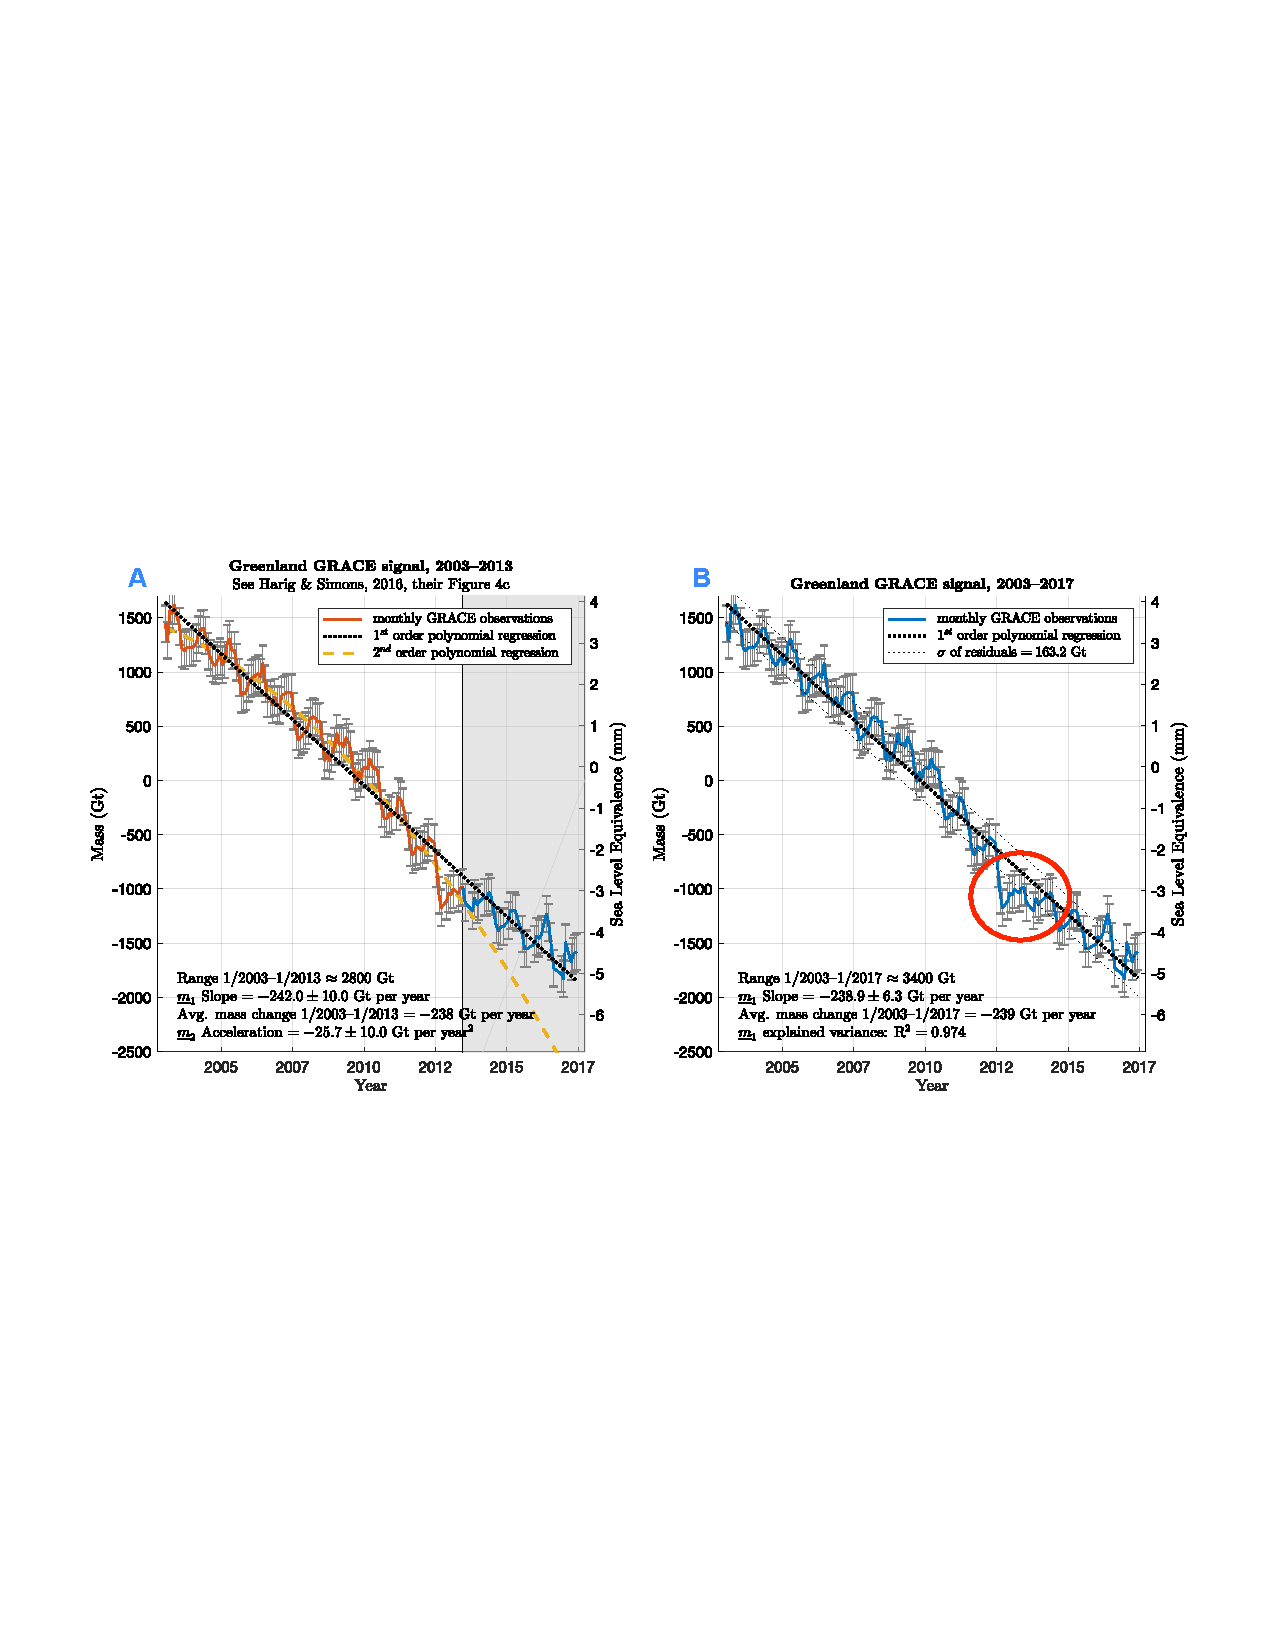
\includegraphics[height=0.37\textheight]
{Figures/HarigGetraerTrend.pdf}}
\caption[Greenland Mass Trend: 2003--2017]{Total mass changes for Greenland over the complete GRACE record using equivalent methods to \cite{Harig+2016}. Shown in \textbf{A} are the $\underline{m}_1$ (linear) and $\underline{m}_2$ (quadratic) models for 01/2003--06/2013, comparable to previous estimates of the mass trend \citep{Harig+2016}. Note the significant departure of the extrapolated $\underline{m}_2$ model from the continuing signal. Shown in \textbf{B} is the $\underline{m}_1$ linear model for 01/2003--06/2017 with the standard of deviation of its residuals. Note that the $\underline{m}_1$ model does not significantly change after including the entire GRACE record. Error bars represent $2\sigma$ based on the combined variance of modeled Slepian coefficients $f_{\alpha}$ (see \cite{Harig+2016}, as well as \cite{getraerFall,getraerSpring}). This figure appeared in \cite{getraerFall,getraerSpring}, here with minor updates.} \label{fig:Getraer}
\end{figure}

Average global surface temperature is rising at an increasing rate---approximately $0.09\degree$~C per decade since 1880, and approximately $0.26\degree$~C per decade since 1979 \cite[][]{ipcc2013_atmosphere}---with the past five years (2014--2018) being approximately $0.84\degree$~C warmer than the 1880--2018 average \cite[][]{NOAA_stateofclimate}. Earth's warming climate has contributed to significant melting of Earth's cryosphere, including the Greenland Ice Sheet where recent ice loss is estimated at $-244$~Gt per
year \cite[][]{ipcc2013_cryosphere,Harig+2015a,Harig+2016}. 
Global melting of ice sheets and glaciers accounts for almost half of recently observed rising sea levels, with Greenland alone contributing almost $25$\% of the $3$~mm per year of sea level rise observed since 1993
\cite[][]{Nerem}. 



With globally increasing temperatures, it seems logical that melt on the Greenland Ice Sheet would increase each year. However, in the final $5$~years of GRACE data, the initially hypothesized acceleration did not pan out (see Figure~\ref{fig:Getraer}). A high level of melt in the Summer of 2012 was followed by two Summers of very little melting in 2013 and 2014, and the end of the GRACE record does not come close to continuing the initially hypothesized acceleration  \cite[see
Figure~\ref{fig:Getraer} A, comparable to][their
Figure~4]{Harig+2016}. This disruption of the apparent 2003--2012 trend was initially described as a ``departure'' or ``deviation'' \cite[][]{Harig+2016}, and more recently as a ``pause'' \cite[][]{bevis2019}, from the accelerating rate of ice loss. While theoretically the long term trajectory of ice loss in a warming climate would be accelerating, the higher melt years within the 2003--2012 are increasingly being contextualized as inter-annual variability with unknown correlation to broader warming and climate change \cite[][]{mattingly2018,hahn2018,bevis2019}. Previous analysis of the complete GRACE data set (2003--2017) using identical methods to \cite{Harig+2016} shows a linear, not accelerating, trend of ice loss for the Greenland Ice Sheet, constraining unexpected deviations mostly to an unusually large melt Summer in 2012 followed by a Summer of unusually little melt in 2013 (see
Figure~\ref{fig:Getraer} B), both of which were primarily concentrated in the SW of the Greenland Ice Sheet (see Figure~\ref{fig:deviant}). 

\begin{wrapfigure}{r}{0.5\textwidth} 
%\vspace{-40pt}
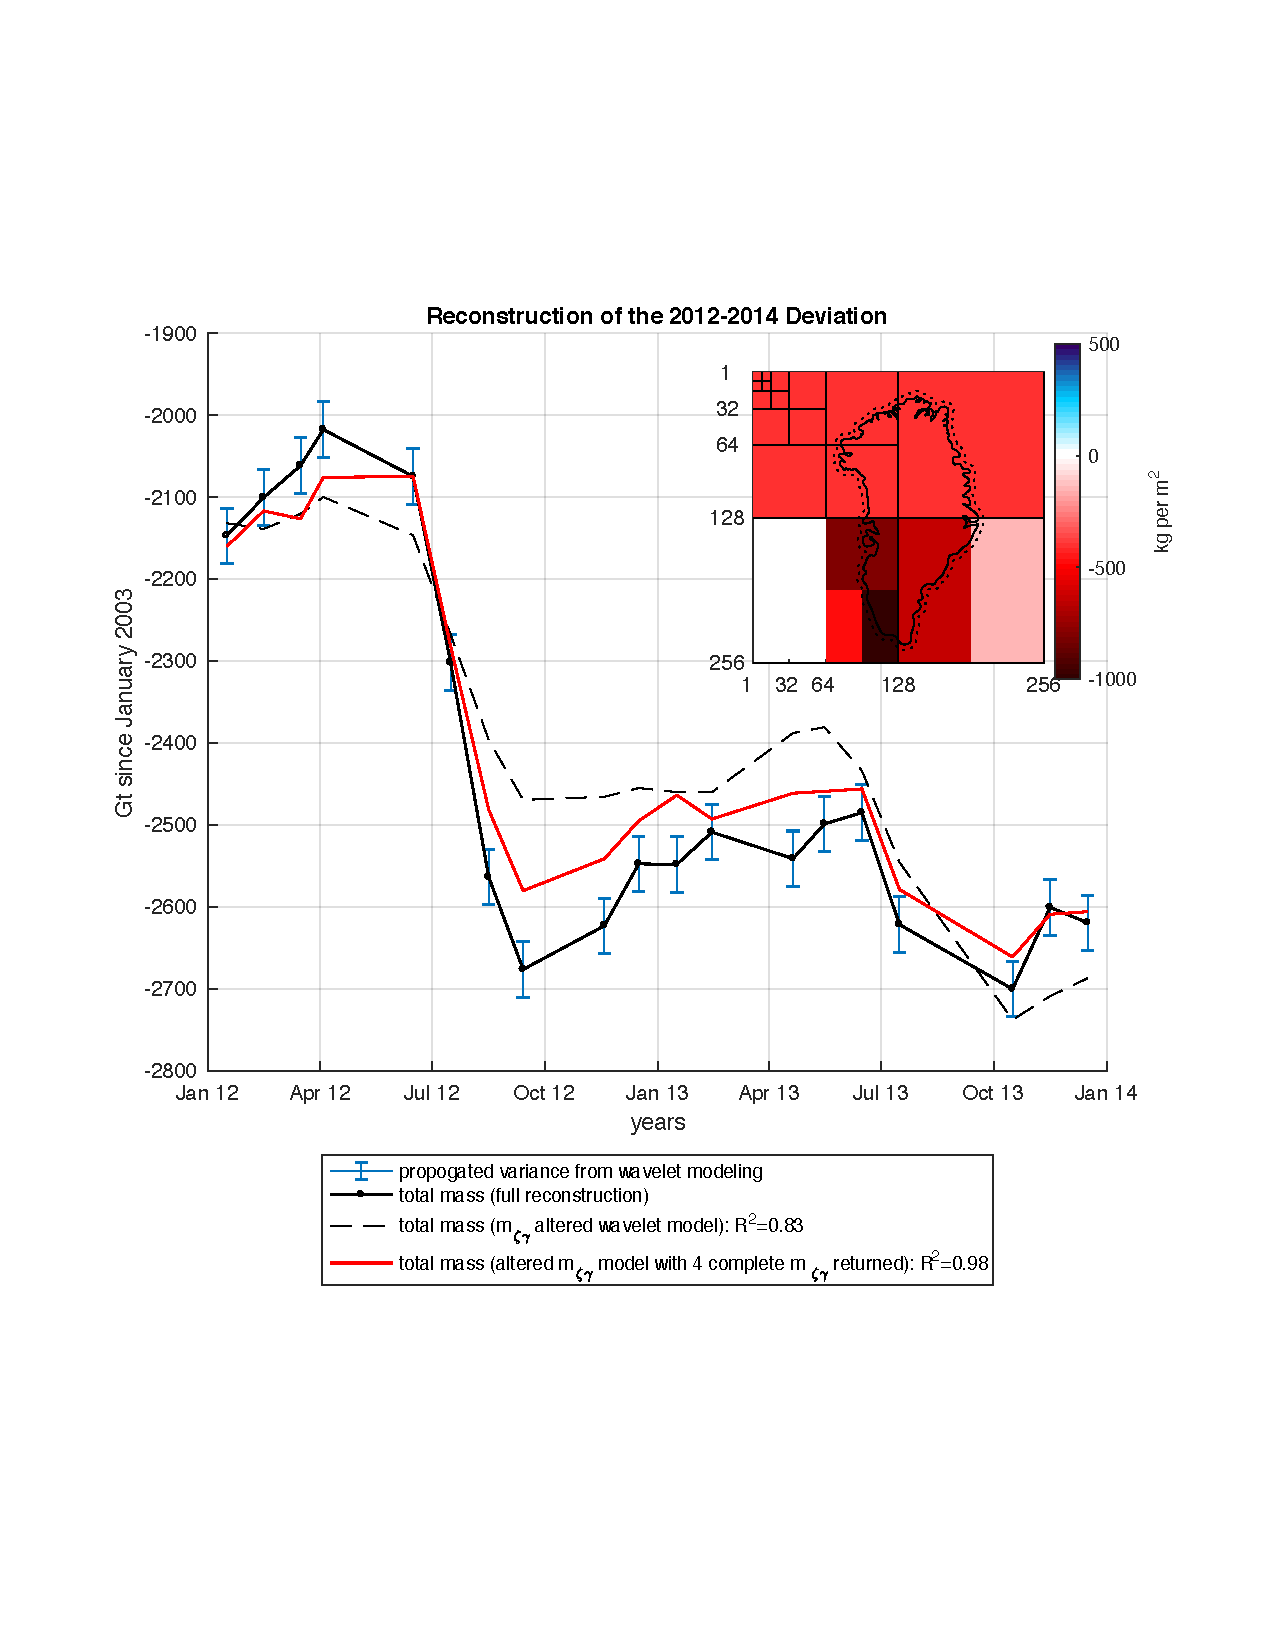
\includegraphics[width=\linewidth]{Figures/deviant.pdf}
\caption[Location of the 2012--2014 Deviation]{The 2012--2014 deviation in Greenland mass (solid black) and the total from a 2-D wavelet based model (dashed black, see \nameref{app:b}). Note the large residual gap between the two lines from July~2012--July~2013, after the anomalously large melt season of 2012. By returning in the actual values of only four wavelet coefficients to the modeled wavelet reconstruction we improve the variance of the residuals by $15\%$. These wavelets are shown inset, colored as a heat map by their coefficient weights in September 2012 (the extreme of the deviation) and are concentrated in southwestern Greenland. ``m$_{\zeta\gamma}$'' refers to a wavelet basis function ``m'' of index $\gamma$ in level $\zeta$. This Figure appeared in my Spring JP.
\label{fig:deviant}}
\end{wrapfigure}

Annual change in total ice mass is generally determined by a combination of discharge from calving glacier termini at the edges of
the ice sheet and by surface mass-balance, the difference between
seasonal snow accumulation and melting \cite[][]{khan2015,enderlin2014}.
Significant inter-annual variability and inter-regional asynchronicity has been observed in the discharge rates of the Greenland Ice Sheet's major drainage basins, while
surface mass-balance has seemed comparatively more predictable
\cite[][]{mcmillan2016,enderlin2014}. The anomalous seasons of 2012--2013 have received attention in recent literature by studies attempting to understand how surface mass-balance processes produce such inter-annual variability. Correlations have been found with climate indices such as the phase of the North Atlantic Oscillation (NAO) \cite[][]{mcmillan2016,bevis2019,hahn2018,getraerFall}; transient atmospheric transport of warm air and water vapor in so-called "atmospheric rivers" \citep{mattingly2018}; non-radiative energy flux enhanced by short-term cloud cover \citep{solomon2017}; as well as albedo and net downward short-wave radiation flux \citep{angelen2014}.  These theories generally relate to variability in atmospheric circulation over Greenland, demonstrating that certain conditions which enhance melt tended to occur more frequently than usual bewteen 2003--2012, and were especially strong during the 2012 melt season. 




\begin{figure}[h]
\centering
\makebox[\textwidth][c]{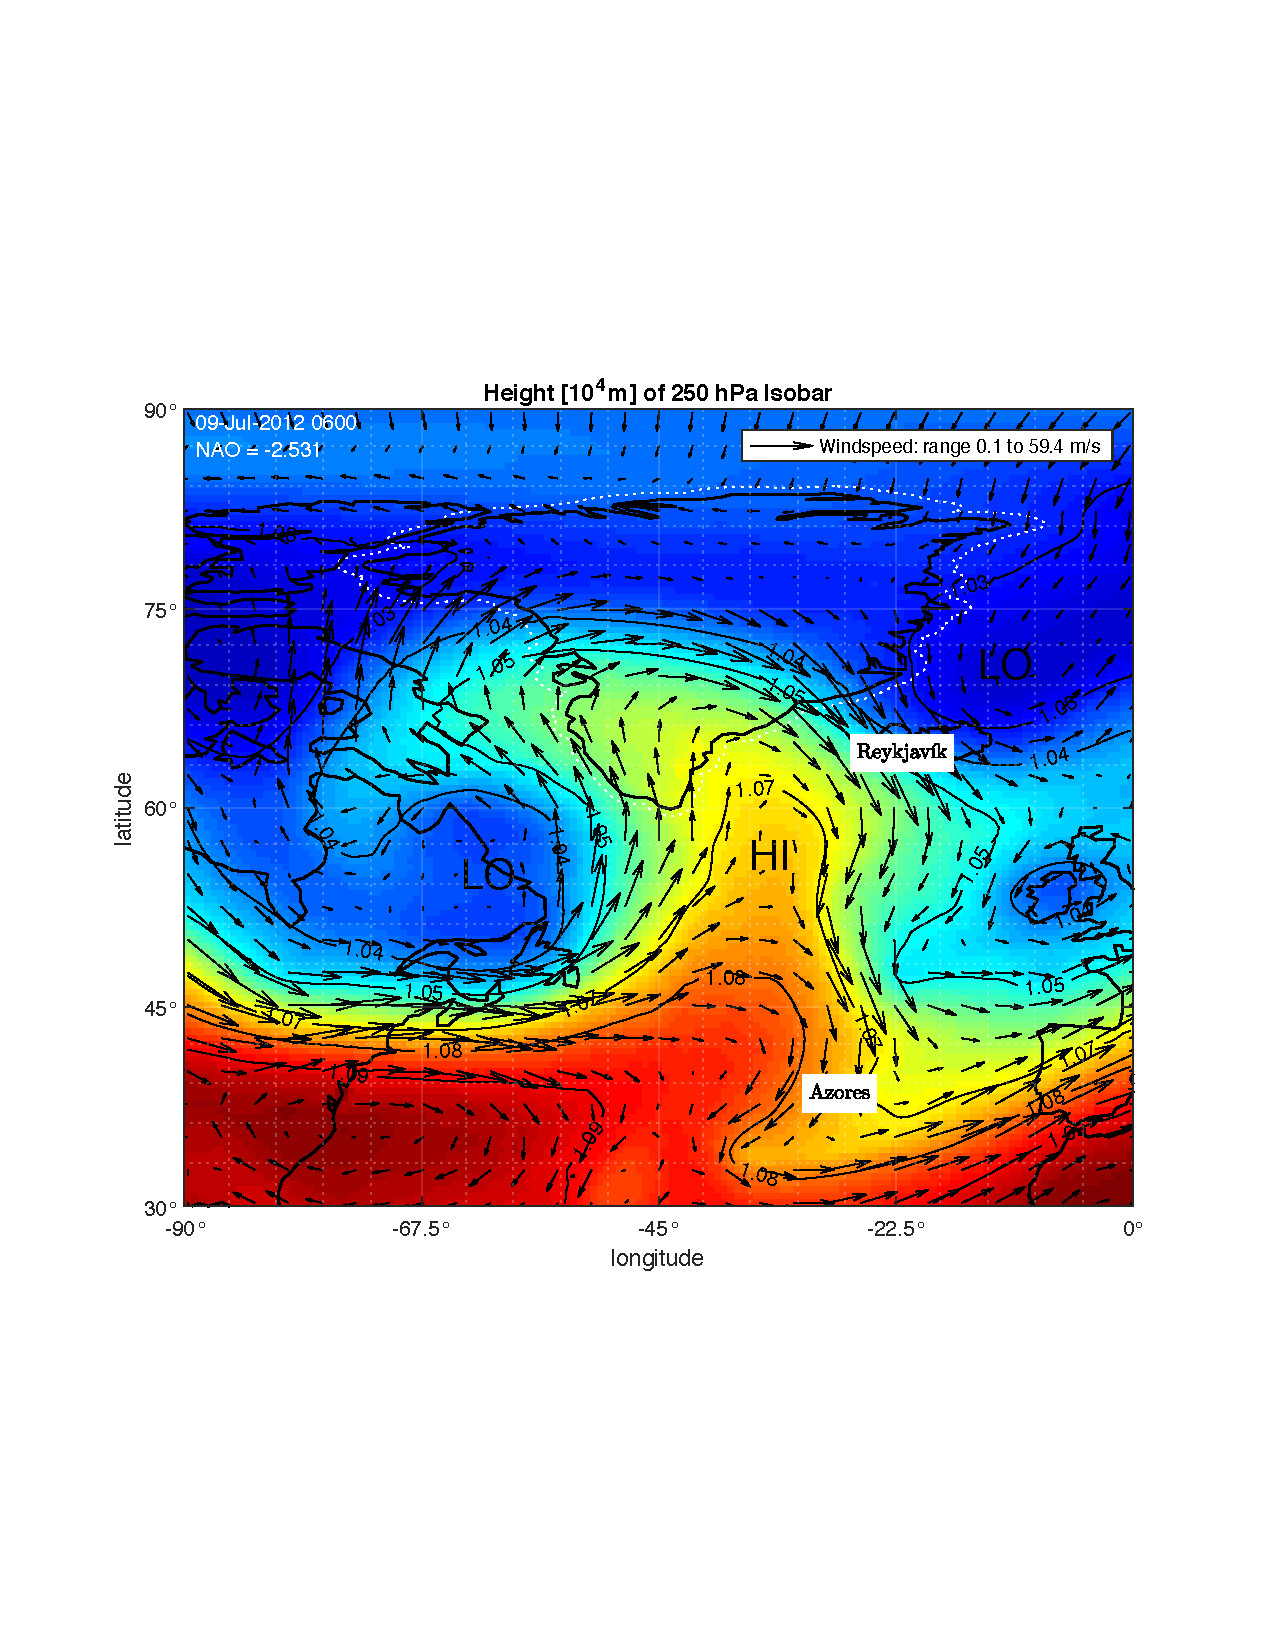
\includegraphics[height=0.5\textheight]
{Figures/jetstream.pdf}}
\caption[Atmospheric Circulation Around Greenland]{Example of atmospheric conditions at the $250$~hPa isobar over the North Atlantic preceding record Greenland Ice Sheet surface melt, 07/09/2012 (from MERRA-2 reanalyzed data). Isobar height contours are labeled in $10^4$~m, and wind vectors are shown by arrows. Note the location of the northern polar jet stream, dividing the low and high isobar heights around the $1.05\times 10^{4}$~m contour. The temporary North Atlantic Rossby wave is labeled as the ``HI'' pressure anti-cyclone moving north towards southern Greenland, with a complementary ``LO'' pressure cyclone centered over Labrador. Note that the jet stream is deflected through the Labrador Sea and Baffin Bay, along the West Coast of Greenland. As a result of these conditions, the ``LO'' pressure over Reykjav\'ik is pushed north, and the pressure difference between Reykjav\'ik  and Azores is lowered, resulting in an negative NAO index (top left).} \label{fig:jetstream}
\end{figure}



%% SIGNIFICANCE OF THE POLAR JET STREAM
\subsection{Atmospheric Circulation Over the Greenland Ice Sheet}
The atmospheric circulation affecting the Greenland Ice Sheet is broadly controlled by the position of the polar jet stream in the northern hemisphere \cite[][]{hanna2013,mattingly2018}. The northern polar jet stream is a strong current of air moving generally eastward, dividing the warm, high pressure air of the temperate mid-latitudes and the cold, low pressure air of the Arctic. In the North Atlantic, the average position of the polar jet results in a low pressure Arctic system centered near Iceland, and a high pressure temperate system centered near the Azores. The strength of the polar jet stream moving air zonally across the North Atlantic is determined by the relative meridional pressure difference across the North Atlantic, and varies irregularly in what is called the North Atlantic Oscillation (NAO) \cite[][]{hurrelNAO}.

%The NAO is often indexed for use in climate analyses by differencing the atmospheric pressure over the North Atlantic and a "loading pattern" of pressure determined by principal component analysis to capture the average meridional pattern \cite[][]{hurrelNAO,cpcNAO}. A positive phase NAO index reflects a stronger meridional difference in pressure than usual, while negative values reflect a weaker meridional difference than usual \cite[][]{hurrelNAO}. %The index is a unitless ratio normalized by the variance of atmospheric pressure from the loading pattern.

%In studying melt events on the Greenland Ice Sheet, many studies have used an NAO index to relate melting conditions to atmospheric pressure patterns. Strong Summer melt events often occur with a negative NAO index, suggesting that mechanisms which drive the NAO may have some kind of predictable implications for melting on Greenland \cite[][]{hanna2013,mattingly2018,mcmillan2016,bevis2019,getraerFall,hahn2018}. More precisely, the use of the NAO index suggests that meridional pressure differences which drive westerly winds across the North Atlantic are a physical mechanism for strengthening melt conditions over Greenland --- warm, moist air, and increased cloud cover \cite[][]{hanna2013,mattingly2018,mcmillan2016,bevis2019,getraerFall,hahn2018}. This assumption, however, obscures the fact that melt events are often caused by southerly winds advecting atmospheric rivers of warm, moist air north, which is driven by a zonal difference in pressure \cite[][]{hanna2013,mattingly2018}. Although the NAO loading pattern for some months suggest southwesterly winds, it is not designed to best capture the type of pattern associated with greater melting events.


The polar jet does not maintain stable zonal flow, and regularly develops instabilities in which flow is diverted meridionally in large waves. During these events, known as a Rossby waves, temporary high-pressure systems push northward into the arctic accompanied by complementary low-pressure cyclones which develop on either side of the high-pressure block. The combined flow from these pressure systems advects warm air from the temperate mid-latitudes into the Arctic until the Rossby wave ``breaks'' and the jet stream return to its average location.


In studying melt events on the Greenland Ice Sheet, many studies have used an NAO index to relate melting conditions to atmospheric pressure patterns. Strong Summer melt events often occur with a negative NAO index, suggesting that mechanisms which drive the NAO may have some kind of predictable implications for melting on Greenland \cite[][]{hanna2013,mattingly2018,mcmillan2016,bevis2019,getraerFall,hahn2018}. However, melt mechanisms such as atmospheric rivers advecting warm moist air over the ice sheet are related to zonal differences in pressure resulting from Rossby wave systems with high pressure ``blocking'' over southern Greenland \cite[][]{mattingly2018}. In contrast, the NAO index measures against a meridional patterns of pressure, with the result that although melt events often correspond with a weaker NAO, a lower the NAO index does not strictly imply a greater melt event (Figure~\ref{fig:naovt}).

\begin{figure}[h]
\centering
\makebox[\textwidth][c]{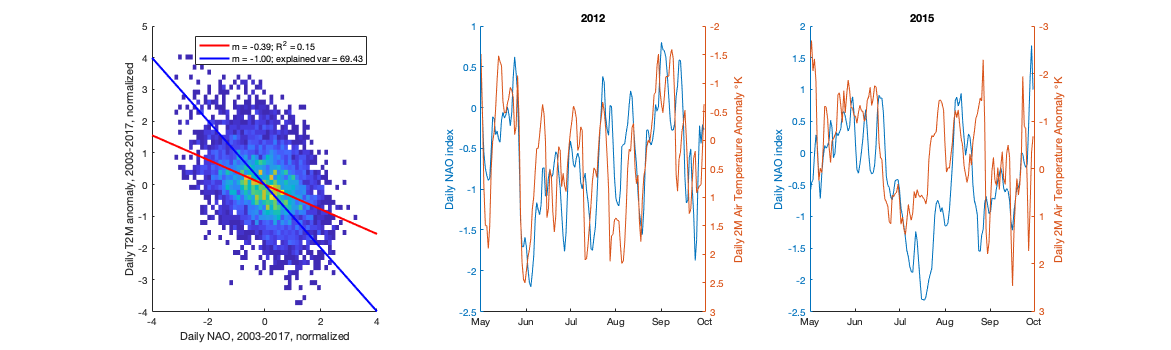
\includegraphics[width=1\linewidth]
{/Users/benjamingetraer/Documents/IndependentWork/senior-thesis/figures/spring2019/NAOvAirT.png}}
\caption[NAO vs. Near surface air temperature: 2003--2017]{Comparison of daily NAO index values to mean daily near surface temperature anomaly over the Greenland Ice Sheet, 2003--2017 (see Section:~\ref{sec:data}~\& \nameref{app:a}). The scatter plot of values in \textbf{A} is binned and colored by concentration of values (blue is low, yellow is high), and shows a type-1 LSR linear fit in red, representing the fit which characterizes a relationship of temperature determined by the NAO index. The LSR fit is influenced by the orientation of the values concentrated towards the center of the plot. The blue line is the first principal component of the two data vectors, showing the single axis which best minimizes the variance of the scattered values. Note that both show a negative correlation (i.e. lower NAO relating to higher 2m air temperatures over the Greenland Ice Sheet), but the PCA fit better captures the overall extent of the data scatter, and shows almost a $1$:$1$ relationship. The variance of the data around these fit lines is illustrated in plots \textbf{B} and \textbf{C}, which show the timeseries of the two values over the 2012 and 2015 Summers. Note that in 2012, NAO and T2M correlated quite closely, while in 2015, there is far less of a connection and the lowest NAO values do not correspond to the highest temperatures.} \label{fig:naovt}
\end{figure}

High pressure blocking over southern Greenland is often correlated with a negative NAO index, because the northern excursion of high pressure systems influences meridional pressure balance. However, despite their correlation, the two are fundamentally different atmospheric patterns which drive advection of air in different directions. In some recent studies, the Greenland Blocking Index (GBI) has been used, which is essentially the average pressure over Greenland. While this is more specific and more relevant than the NAO index, it still does not directly reflect the meridional advection which drives melt.

The search for an easily definable index which captures atmospheric circulation patterns that drive melt fell outside of the scope of this project. Circulation patterns provide important context for the variability of weather events, but here I return to the more fundamental question of surface level melt processes. While the majority of energy that is absorbed by melting ice comes from solar radiation and processes which amplify insolation \cite[][]{mattingly2018, solomon2017,angelen2014}, near surface temperature broadly determines the regions which will be melting at any given time \cite[][]{broeke2011}. 

In this paper, I examine trends near surface temperature between 1980--2017 and correlation of near surface temperature to mass anomaly between 2003--2017 in order to provide context to previous results which have been examining the variability in mass loss and atmospheric forcings over the past two decades. While a few studies have examined direct relationships between temperature and melting, comparisons connect to melt maps generated through passive microwave observation from satellites, and are do not examine the direct relationship to mass loss data such as GRACE \cite[][]{cullather2018,valisuo2018}.



 
 
% These atmospheric conditions are illustrated in Figure~\ref{fig:jetstream}, illustrating the Greenland blocking event in July 2012, immediately preceding record surface melting on the Greenland Ice Sheet on 07/11/2012 \cite[][]{hanna2013,mattingly2018}.



%The conclusion of many studies would be to suppose that the NAO is driving Greenland melt, and to look to patterns in the NAO index to understand the future of Greenland's ice sheet. This is highly concerning, as there are strong signs that the NAO has been trending more and more negative in recent years. However, it is crucial to note that there are significant theoretical obstacles in the correlation of the NAO index to melt. 



%The general conclusions drawn by these studies point to common atmospheric processes of uncommon duration or intensity. 







%In my Spring 2018 JP, I explored the use of a 2-D wavelet basis to represent the GRACE gravimetric data over Greenland such that meaningfully contributing basis functions also contained information about spatial structure (see
%Figure~\ref{fig:}). 
%
%I developed a procedure for choosing the most important wavelet basis functions in order to extract the true fluctuation of the signal from the over-determined image calculated from the typical GRACE spherical harmonic basis. I then tested which wavelet basis function best captured the 2012--2013 deviation from the expected signal, finding the deviations to be concentrated in southwestern Greenland (see
%Figure~\ref{fig:deviant}). 



%%%%%%%%%%%%%%%%%%%%%%%%%%%%%%%%%%%%%%%%%%%%%%%%%%%%%%%%%%%%%%%%%%%%%%%%%%%%%%%%%%%%%%%%%%%%%%%%%%%%%%%%%%%%%%%%%%%%%%%%%%%%%%%%%%%%%%%%%%%%%%%%%%%%%%%%%%%%%%%%%%%%%%%%%%%%%%%%%%%%
%% SECTION: DATA
%%%%%%%%%%%%%%%%%%%%%%%%%%%%%%%%%%%%%%%%%%%%%%%%%%%%%%%%%%%%%%%%%%%%%%%%%%%%%%%%%%%%%%%%%%%%%%%%%%%%%%%%%%%%%%%%%%%%%%%%%%%%%%%%%%%%%%%%%%%%%%%%%%%%%%%%%%%%%%%%%%%%%%%%%%%%%%%%%%%%
\section{Data \label{sec:data}}

\subsection{Ice Mass Data}

Observations of ice loss across large areas are measured remotely by satellites using several different methods, including weighing the mass by gravitational anomaly (such as NASA's GRACE and GRACE Follow-On missions), photographing surface area (such as NASA's \href{https://landsat.gsfc.nasa.gov}{Landsat} and \href{https://terra.nasa.gov/about/terra-instruments/modis}{MODIS} missions), and by measuring relative height of the ice with active laser altimetry (such as NASA's \href{https://icesat.gsfc.nasa.gov/icesat/}{ICESat} and \href{https://icesat-2.gsfc.nasa.gov}{ICESat-2} missions) \cite[][]{khan2015}.

Data used in this study come from the GRACE satellite mission, span from 2003--2017, and were released as global spherical harmonic coefficients by NASA in the CSR-RL05 data product (see \nameref{app:a}; for an in depth review of GRACE data reduction methods, see \nameref{app:b}). For this project, the RL05 spherical harmonic coefficients were evaluated directly onto the analysis grid (see Figure~\ref{fig:gridbasins}).
 
 \subsection{Atmospheric Data}
 
 
In addition to datasets which directly measure physical manifestations of ice sheet melting, there are complimentary datasets which capture some of the processes which control melting such as air temperature, humidity, and cloud cover. The primary atmospheric data used in this study are reanalysis products from the Modern-Era Retrospective analysis for Research and Applications, Version 2 (MERRA-2) (see Table~\ref{tab:merradata} and \nameref{app:a}). 

%%%%%%%%%%%%%%%%%%%%%%%%%%%%%%%%%%%%%%%%%%%%%%%%%%%%%%%%%%%%%%%%%%%%%%%%%%%%%%%%%%%%%%%%%%%%%%%%%%%%%%%%%%%%%%%%%%%%%%%%%%%%%%%%%%%%%%%%%%%%%%%%%%%%%%%%%%%%%%%%%%%%%%%%%%%%%%%%%%%%
%% MERRA-2 DATA TABLE
%%%%%%%%%%%%%%%%%%%%%%%%%%%%%%%%%%%%%%%%%%%%%%%%%%%%%%%%%%%%%%%%%%%%%%%%%%%%%%%%%%%%%%%%%%%%%%%%%%%%%%%%%%%%%%%%%%%%%%%%%%%%%%%%%%%%%%%%%%%%%%%%%%%%%%%%%%%%%%%%%%%%%%%%%%%%%%%%%%%%
\begin{table}[!h]
\begin{center}
\begin{tabular}{ |l|c|l| } 
\hline
\bfseries{Variable} & \bfseries{Temporal Resolution} & \bfseries{Dataset}\\
\hline
2 Meter Air Temperature 			& daily 	&  tavg1\_2d\_slv\_Nx\\ 
									& monthly 	&  statM\_2d\_slv\_Nx\\
500 hPa Air Temperature 			& daily 	&  tavg1\_2d\_slv\_Nx\\ 
2 Meter Air Specific Humidity 		& daily 	& tavg1\_2d\_slv\_Nx \\ 
500 hPa Air Specific Humidity 		& daily 	& tavg1\_2d\_slv\_Nx \\ 
Skin Surface Temperature 			& daily 	& tavg1\_2d\_slv\_Nx \\ 
Total Cloud	Area Fraction			& daily 	& tavg1\_2d\_rad\_Nx \\
Surface Net Downward Shortwave Flux & daily 	& tavg1\_2d\_rad\_Nx \\
\hline
\end{tabular}
\caption[MERRA-2 Data]{MERRA-2 data used in this study (see \nameref{app:a}). Mean daily and monthly values were accessed on the default MERRA-2 $0.625^{\circ}$~lon$\times0.5^{\circ}$~lat grid with an original spatial resolution of approximately $50$~km$\times50$~km\cite[][]{bosilovich2016}. Values are based on the GEOS climate models which combine direct observations into a globally continuous representation of the atmosphere, ocean, and surface interactions using a consistent set of of conservation assumptions \cite[][]{gelaro2017,bosilovich2016}. \label{tab:merradata}}
\end{center}
\end{table}
%%%%%%%%%%%%%%%%%%%%%%%%%%%%%%%%%%%%%%%%%%%%%%%%%%%%%%%%%%%%%%%%%%%%%%%%%%%%%%%%%%%%%%%%%%%%%%%%%%%%%%%%%%%%%%%%%%%%%%%%%%%%%%%%%%%%%%%%%%%%%%%%%%%%%%%%%%%%%%%%%%%%%%%%%%%%%%%%%%%%
%%%%%%%%%%%%%%%%%%%%%%%%%%%%%%%%%%%%%%%%%%%%%%%%%%%%%%%%%%%%%%%%%%%%%%%%%%%%%%%%%%%%%%%%%%%%%%%%%%%%%%%%%%%%%%%%%%%%%%%%%%%%%%%%%%%%%%%%%%%%%%%%%%%%%%%%%%%%%%%%%%%%%%%%%%%%%%%%%%%%

``Reanalysis'' refers to a way of processing an ensemble of directly measured weather observations using a consistent set of rules that assume physical constraints on the ways in which different atmospheric variables interact temporally and spatially \cite[][]{gelaro2017}. These physical constraints are defined by a global climate model, which can both make forecasts of future developments of meteorological variables and output modeled solutions based on weather measurements directly observed at weather stations all over the world \cite[][]{gelaro2017}. Variable values for a given time and spatial location are calculated as a best fit of direct observations to the constraints of multiple different models which define processes such as radiation balances, physical movement, chemical interactions, precipitation, and so forth, or are inferred by the models' rules from variables which are directly measured \cite[][]{bosilovich2016,gelaro2017}.  

The data for this study come from NASA's Global Modeling and Assimilation Office's Goddard Earth Observing System (GEOS) climate models, and are publicly available in specific MERRA-2 data products through the NASA Goddard Earth Sciences Data Information Services Center (GES DISC) (see \nameref{app:a}). MERRA-2 data are available in several different spatial and temporal formats for different variables. I use gridded daily averages for examining the connections between meteorological variables over the Greenland Ice Sheet, and gridded monthly averages for capturing the long-term development of Greenland's climate. Daily and monthly data are taken from collections of single-level, two-dimensional data which GES DISC provides in a few MERRA-2 datasets (see Table~\ref{tab:merradata}, \nameref{app:a}).
 

Daily and monthly NAO climate index values are provided by the National Weather Service Climate Prediction Center, which calculates NAO index values from the $500$~mb pressure level height over the spatial extent of $20$--$90^{\circ}$~N \cite[][]{cpcNAO}. Pressure level heights are compared to a monthly loading pattern defined as the first principal component of a rotated principal component analysis on the 1950--2000 $500$~mb height time-series and values are normalized by monthly mean and standard of deviation for the 1950--2000 index time-series \cite[see \nameref{app:a} and][]{cpcNAO}.

Lastly, Northern Hemisphere climate data are from the Goddard Institute for Space Studies Surface Temperature Analysis (GISTEMP v3) as a mean monthly Land-Ocean Temperature Index (LOTI), which takes into account dampening of atmospheric temperature changes due to the heat capacity of ocean water \cite[][]{hansen2010}. The data used here are a monthly index of temperature anomalies from 1951--1980 time-series, which are available from 1880--present \cite[see \nameref{app:a} and][]{hansen2010}.


%%%%%%%%%%%%%%%%%%%%%%%%%%%%%%%%%%%%%%%%%%%%%%%%%%%%%%%%%%%%%%%%%%%%%%%%%%%%%%%%%%%%%%%%%%%%%%%%%%%%%%%%%%%%%%%%%%%%%%%%%%%%%%%%%%%%%%%%%%%%%%%%%%%%%%%%%%%%%%%%%%%%%%%%%%%%%%%%%%%%
%% Methods
%%%%%%%%%%%%%%%%%%%%%%%%%%%%%%%%%%%%%%%%%%%%%%%%%%%%%%%%%%%%%%%%%%%%%%%%%%%%%%%%%%%%%%%%%%%%%%%%%%%%%%%%%%%%%%%%%%%%%%%%%%%%%%%%%%%%%%%%%%%%%%%%%%%%%%%%%%%%%%%%%%%%%%%%%%%%%%%%%%%%
 \section{Methods}
 
All analysis of MERRA-2 data over the Greenland Ice Sheet was masked using a widely used shape-file of the ice sheet developed from the drainage subregions defined by \cite{zwally2012}, reorganized into quadrants similar to \cite{mcmillan2016} (see Figure~\ref{fig:gridbasins}). Anomaly values were calculated by subtracting the mean value for that month relative to the given period being examined. Seasonal values are the mean of all values falling within the months of that season, defined as Winter (December-January-February), Spring (March-April-May), Summer (June-July-August), and Fall (September-October-November). Comparisons of mass anomaly and MERRA-2 variables were done on the analysis grid described in Figure~\ref{fig:gridbasins}, using bi-linear interpolation to sample the MERRA-2 variables. Spatially heterogeneous trends were analyzed by modeling the anomaly of each point on the analysis grid through time (e.g. Figure~\ref{fig:tslopes}). 

%%%%%%%%%%%%%%%%%%%%%%%%%%%%%%%%%%%%%%%%%%%%%%%%%%%%%%%%%%%%%%%%%%%%%%%%%%%%%%%%%%%%%%%%%
% Basins figure
%%%%%%%%%%%%%%%%%%%%%%%%%%%%%%%%%%%%%%%%%%%%%%%%%%%%%%%%%%%%%%%%%%%%%%%%%%%%%%%%%%%%%%%%%
\begin{figure}[h]
\centering
\makebox[\textwidth][c]{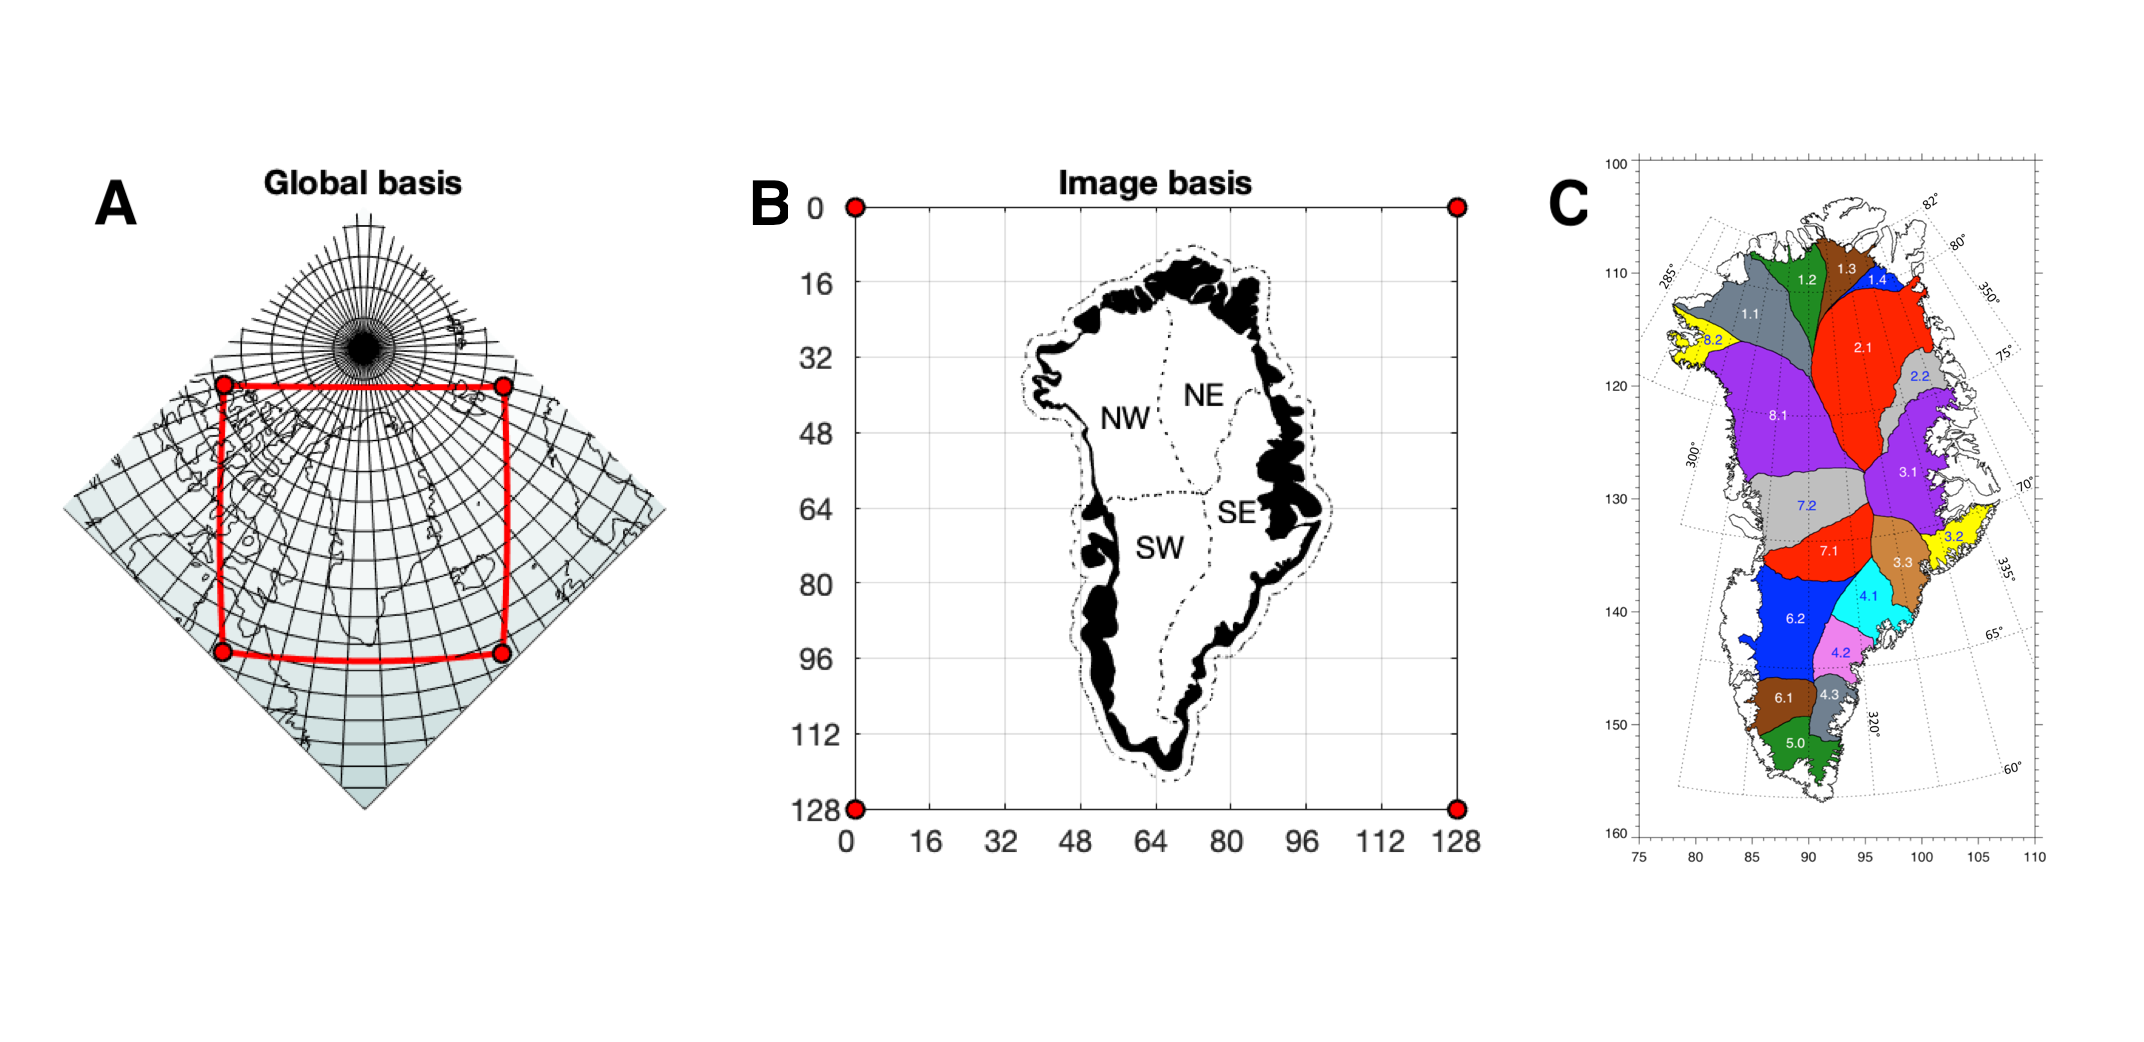
\includegraphics[width=1.1\linewidth]{/Users/benjamingetraer/Documents/IndependentWork/senior-thesis/figures/spring2019/gridandbasins.png}}
\caption[The Discrete Grid Around Greenland]{I defined a grid in the global basis on a face of the \textit{Cubed Sphere} centered on Greenland (\textbf{A}), upon which the I evaluate gravitational anomaly from GRACE spherical harmonic solutions, and interpolate MERRA-2 data for comparison \cite[see][]{ronchi1996}. In the image basis (\textbf{B}) the grid is cartesian with length $128$. The filled black area is the island of Greenland, with the extent of the ice sheet superimposed in white, and dotted lines delineating the regional quadrants that we consider \cite[see \textbf{C}~\&][]{zwally2012}. Dotted around Greenland is a coastal buffer of $0.5^{\circ}$, within which the total Greenland mass budget from GRACE is integrated, as in \cite{Harig+2016}. Points on the grid are approximately $20$--$25$~km apart, finer than both GRACE and MERRA-2 spatial resolutions. Drainage subregions of Greenland used to define ice sheet extent and quadrants in this paper are derived from \textbf{C} \cite[figure and data from][]{zwally2012}. Quadrants shown in \textbf{B} are unions of these subregions as follows: NW~$=\cup(1.1, 1.2)$; NE~$=\cup(1.3, 1.4, 2.1, 2.2)$; SE~$=\cup(3.1, 3.2, 3.3, 4.1, 4.2, 4.3)$; SW~$=\cup(5.0,6.1,6.2,7.1,7.2)$, similar to the divisions made in \cite{mcmillan2016} \label{fig:gridbasins}}
\end{figure}
%%%%%%%%%%%%%%%%%%%%%%%%%%%%%%%%%%%%%%%%%%%%%%%%%%%%%%%%%%%%%%%%%%%%%%%%%%%%%%%%%%%%%%%%%%%%%%%%%%%%%%%%%%%%%%%%%%%%%%%%%%%%%%%%%%%%%%%%%%%%%%%%%%%%%%%%%%%%%%%%%%%%%%%%%%%%%%%%%%%%

 %%%%%%%%%%%%%%%%%%%%%%%%%%%%%%%%%%%%%%%%%%%%%%%%%%%%%%%%%%%%%%%%%%%%%%%%%%%%%%%%%%%%%%%%%%%%%%%%%%%%%%%%%%%%%%%%%%%%%%%%%%%%%%%%%%%%%%%%%%%%%%%%%%%%%%%%%%%%%%%%%%%%%%%%%%%%%%%%%%%%
%% RESULTS
%%%%%%%%%%%%%%%%%%%%%%%%%%%%%%%%%%%%%%%%%%%%%%%%%%%%%%%%%%%%%%%%%%%%%%%%%%%%%%%%%%%%%%%%%%%%%%%%%%%%%%%%%%%%%%%%%%%%%%%%%%%%%%%%%%%%%%%%%%%%%%%%%%%%%%%%%%%%%%%%%%%%%%%%%%%%%%%%%%%%
 \section{Results}
 
 \subsection{Near Surface Temperature Trends Since 1980}
 
 Over the 1980--2017 time period the Northern Hemisphere has been gradually warming, and averaging across the monthly LOTI anomaly with 10~year moving window reveals a quite linear trend of $0.24^{\circ}$C per decade (type 1 least-squares regression, with a variance reduction $\mathrm{R^2}=0.987$), for a total increase of $0.89^{\circ}$C since 1980 (see Figure~\ref{fig:climatewarming}). Over the same time period, near surface temperature anomalies over the Greenland Ice Sheet had a significantly different pattern of increase, remaining static through the 1980's and more recently since the early 2000's, and increasing dramatically through the 1990's (Figure~\ref{fig:climatewarming}). Comparing the first 15 years (1980--1994) of the 1980--2017 time period to the last 15 years (2003--2017), the mean temperature rose $1.53\pm0.42^{\circ}$C as illustrated in Figure~\ref{fig:climatewarming} (two sample $t$-test found distributions of significantly different mean values, $p = 2.3\mathrm{e}{-12}$; reported error represents the $95\%$ confidence interval on the difference in mean values). 
 
 %%%%%%%%%%%%%%%%%%%%%%%%%%%%%%%%%%%%%%%%%%%%%%%%%%%%%%%%%%%%%%%%%%%%%%%%%%%%%%%%%%%%%%%%%%
%	TOTAL CLIMATE CHANGE FIGURE
%%%%%%%%%%%%%%%%%%%%%%%%%%%%%%%%%%%%%%%%%%%%%%%%%%%%%%%%%%%%%%%%%%%%%%%%%%%%%%%%%%%%%%%%%%
 \begin{figure}[h]
\centering
\makebox[\textwidth][c]{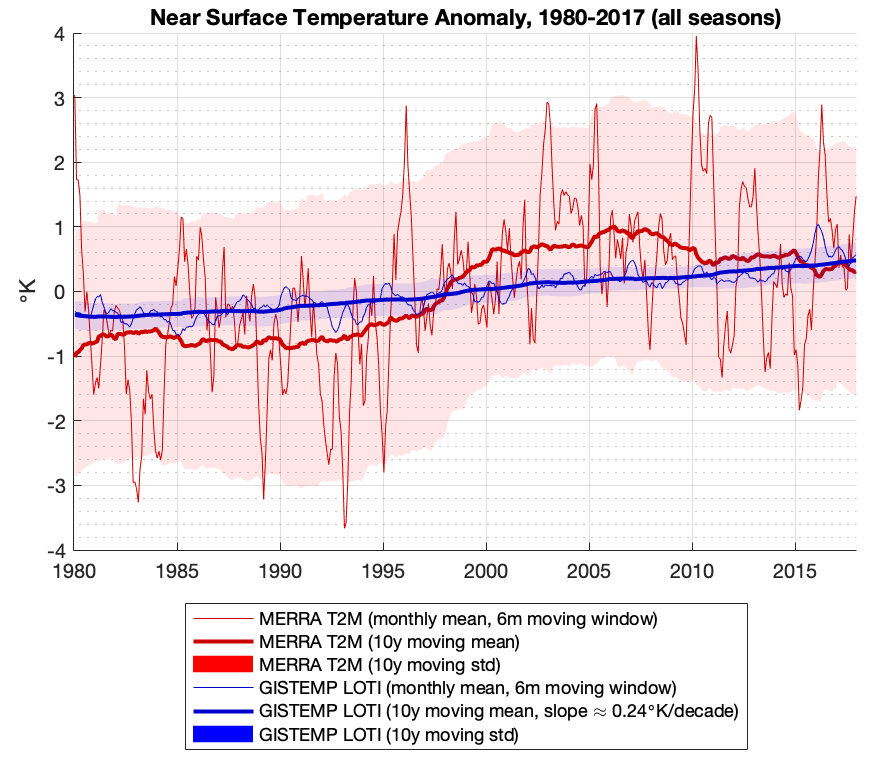
\includegraphics[height=0.5\textheight]
{/Users/benjamingetraer/Documents/IndependentWork/senior-thesis/figures/spring2019/GRISvNHsurfaceT.png}}
\caption[Near surface warming of the Northern Hemisphere and Greenland Ice Sheet]{Mean monthly near surface temperature anomalies for the Northern Hemisphere (GISTEMP Land-Ocean Temperare Index, blue) and the Greenland Ice Sheet (MERRA-2 2m air temperature, red), 1980--2017. Data has been filtered using 6-month and 10-year moving windows for ease of interpretation, with the shaded area representing the spread of the data using the standard of deviation of the 10-year moving window. Note the more continuously linear increase in Northern Hemisphere temperature over the entire time-period compared to the non-linear jump in temperature over Greenland in the 1990's. Analyses of the unfiltered time-series show that: the Northern Hemisphere LOTI is increasing at $0.24^{\circ}$C per decade ($\mathrm{R^2}=0.987$); near-surface air temperature increased $1.53\pm0.42^{\circ}$C between the years 1980--1994 and 2003--2017.} \label{fig:climatewarming}
\end{figure}
%%%%%%%%%%%%%%%%%%%%%%%%%%%%%%%%%%%%%%%%%%%%%%%%%%%%%%%%%%%%%%%%%%%%%%%%%%%%%%%%%%%%%%%%%%


Rise in near surface air temperature across the Greenland Ice Sheet between 1980--2017 differed seasonally, with the greatest rise in temperature occurring in the Winter season (December, January, February) and the smallest rise in temperature occuring in the Summer season (June, July, August) (see Figure~\ref{fig:seasonalclimate}). The fitted linear trends were tested for significance against the hypothesis that a trend of the same magnitude could be generated from similar random data (normally distributed data of the same mean, standard of deviation, and number of points). $p$-values for the trends represent the percentage of trends of greater magnitude found in $10000$ tests of similar random data (the trend slope of greatest absolute value would have $p(\mathrm{max}) = 0$, and a trend slope of $0$ would have $p(0) = 1$). A similar method was used to calculate the confidence interval of these trends, by subtracting the linear fit, generating $10000$ tests of similar random data, and finding the $90^{\mathrm{th}}$ and $95^{\mathrm{th}}$ percentile of slope magnitude amongst the random test data. 

For the seasonal near surface air temperature trends between 1980--2017, all were found to be significant at at least the $p < 0.05$ threshold compared to the $10000$ tests of similar random data (see Table~\ref{tab:seasonaltrends}). The difference in trend between Winter and Summer months is significant in the random simulations, with the best fit trend for each falling outside of the $90\%$ confidence interval of the other (see Table~\ref{tab:seasonaltrends}).

%%%%%%%%%%%%%%%%%%%%%%%%%%%%%%%%%%%%%%%%%%%%%%%%%%%%%%%%%%%%%%%%%%%%%%%%%%%%%%%%%%%%%%%%%%%%%%%%%%%%%%%%%%%%%%%%%%%%%%%%%%%%%%%%%%%%%%%%%%%%%%%%%%%%%%%%%%%%%%%%%%%%%%%%%%%%%%%%%%%%
%% Seasonal climate trends slope table
%%%%%%%%%%%%%%%%%%%%%%%%%%%%%%%%%%%%%%%%%%%%%%%%%%%%%%%%%%%%%%%%%%%%%%%%%%%%%%%%%%%%%%%%%%%%%%%%%%%%%%%%%%%%%%%%%%%%%%%%%%%%%%%%%%%%%%%%%%%%%%%%%%%%%%%%%%%%%%%%%%%%%%%%%%%%%%%%%%%%
\begin{table}[!h]
\begin{center}
\begin{tabular}{ |l|c|c|c|c| } 
\hline
\bfseries{Season} & \bfseries{Trend [$^{\circ}$C/decade]} & \bfseries{$95\%$ conf. int.} & \bfseries{$90\%$ conf. int.} & \bfseries{$p$-value}\\              
\hline
\multicolumn{5}{|c|}{\bfseries{1980--2017}} \\
\hline
Winter (DJF)	& $+0.80$	& $\pm0.46$	& $\pm0.38$	& 	0.0015 \\ 	
\hline
Spring (MAM)	& $+0.46$	& $\pm0.36$	& $\pm0.30$	&	0.0163 \\
\hline
Summer (JJA)	& $+0.35$	& $\pm0.17$	& $\pm0.15$	&	0.0002\\
\hline
Fall (SON)	& $+0.48$	& $\pm0.29$	& $\pm0.25$	&	0.0021\\
\hline
\multicolumn{5}{|c|}{\bfseries{2003--2017}} \\
\hline
Winter (DJF)	& $-0.60$	& $\pm 1.12 $	& $\pm 0.93$	& 	0.413 \\ 	
\hline
Spring (MAM)	& $-0.98$	& $\pm 1.11$	& $\pm 0.94$	&	0.105  \\
\hline
Summer (JJA)	& $-0.72$	& $\pm 1.13$	& $\pm 0.94$	&	0.217\\
\hline
Fall (SON)		& $-0.02$	& $\pm 1.13$	& $\pm 0.94$	&	0.971\\
\hline\end{tabular}
\caption[Seasonal 2m temperature trends over the Greenland Ice Sheet: 1980--2017]{Seasonal trends in MERRA-2 2m air temperature calculated on mean monthly data across the Greenland Ice Sheet for the time period 1980--2017 and 2003--2017, shown in Figure~\ref{fig:seasonalclimate}. The trend is the type 1 least squares regression slope of the mean monthly data, and confidence intervals are the results of synthetic data tests analyzing the residuals of the data and the trend line. $p$-values represent the chances of finding a trend slope of equal or greater magnitude in a random sampling of a ``similar'' normal distribution. For 1980--2017, all seasons have trend magnitudes that are significantly different from a random sampling of a ``similar'' normal distribution at the $p < 0.05$ threshold; Winter and Summer seasonal trends are significantly different from each other at the $90\%$ confidence interval; Fall and Spring trends are not significantly different from Summer, and are not well differentiated from Winter. For 2003--2017, Winter and Fall trends are well within expected fits for similar random data, and while the Spring and Summer trends are more unusual, those negative trends are also not significantly differentiable from similar random data in $p$-value or confidence interval. \label{tab:seasonaltrends}}
\end{center}
\end{table}
%%%%%%%%%%%%%%%%%%%%%%%%%%%%%%%%%%%%%%%%%%%%%%%%%%%%%%%%%%%%%%%%%%%%%%%%%%%%%%%%%%%%%%%%%%%%%%%%%%%%%%%%%%%%%%%%%%%%%%%%%%%%%%%%%%%%%%%%%%%%%%%%%%%%%%%%%%%%%%%%%%%%%%%%%%%%%%%%%%%%


Despite the overall rise in temperature since the 1980's, near surface air temperature across the Greenland Ice Sheet was not increasing over the GRACE record (2003--2017) (Figure~\ref{fig:seasonalclimate}). In fact, mean 2m air temperature anomaly over the ice sheet drifted cooler in every season, most markedly in Spring and Summer (see Figure~\ref{fig:seasonalclimate} \& Table~\ref{tab:seasonaltrends}). The cooling drift in temperature from 2003--2017 was analyzed for significance in the same manner as the trends over the entire 1980--2017 record (Table~\ref{tab:seasonaltrends}). The trends in Winter and Fall were indistinguishable from similar random data drawn from a normal distribution of the same mean and standard of deviation, and while the trends in Spring and Summer were more unusual for random variability, they too were poorly differentiated from similar random data in both $p$-value and confidence interval (Table~\ref{tab:seasonaltrends}). 

Taking into consideration the probability of random simultaneous negative drift in 2m air temperature anomaly across all seasons ($\prod_{\mathrm{season}=i} p_i = 0.0091$) it becomes apparent that within the larger, expected warming trend of 1980--present, Greenland experienced an unexpected cooling hiatus during the 2003--2017 GRACE record (see Figure~\ref{fig:seasonalclimate} \& Table~\ref{tab:seasonaltrends}). It is important to note that, regardless of fitted trends, the majority of the 10 warmest seasons of the 1980--2017 record have occurred during the GRACE record ($6/10$ Winters, $8/10$ Springs, $8/10$ Summers, $6/10$ Falls), and for the first decade of GRACE data, all but one Summer season on the Greenland Ice Sheet had mean temperatures above the 1980--2017 average see (Figure~\ref{fig:seasonalclimate} \& Table~\ref{tab:rankedseasons}).

In addition to differences in near surface temperature anomaly trends found in different seasons and decades, there is also significant spatial heterogeneity temperature anomaly trends across the Greenland Ice Sheet. I calculated a linear fit for temperature anomaly at each node of the grid across Greenland (see Figure~\ref{fig:gridbasins}) for years between 1980--2017, from the beginning of GRACE until the end of 2012 (2003--2012), and for the entire GRACE record (2003--2017), illustrated in Figure~\ref{fig:tslopes}. The trends within those three time periods have very different features, characterized by widespread warming in all seasons (1980--2017), general cooling in non-Summer seasons with strong Summer warming in the SW region (2003--2012), and general cooling across the vast majority of the ice sheet in all seasons (2003--2017) (Figure~\ref{fig:tslopes}). 

%The patterns of temperature captured in Greenland averages which are analyzed over decades (see Figures~\ref{fig:climatewarming}~\&~\ref{fig:seasonalclimate}) are important in understanding first order changes occurring in Greenland climate, but fail to capture

Strong warming in the SW during first decade of the GRACE record was followed by a very different pattern of warming in the north and cooling in the south from 2013--2017, resulting in a trend over the entire 2003--2017 period which obscures the temperature anomaly signal in the SW (Figure~\ref{fig:tslopes}). Also of note is that Summer temperature trends differ significantly in both magnitude and spatial pattern from non-Summer trends, which dominate the fitted trends seen when seasons are not considered separately (see Figures~\ref{fig:seasonalclimate}~\&~\ref{fig:tslopes}).


%%%%%%%%%%%%%%%%%%%%%%%%%%%%%%%%%%%%%%%%%%%%%%%%%%%%%%%%%%%%%%%%%%%%%%%%%%%%%%%%%%%%%%%%%%
%	SEASONAL CHANGE FIGURE
%%%%%%%%%%%%%%%%%%%%%%%%%%%%%%%%%%%%%%%%%%%%%%%%%%%%%%%%%%%%%%%%%%%%%%%%%%%%%%%%%%%%%%%%%%
 \begin{figure}[h]
\centering
\makebox[\textwidth][c]{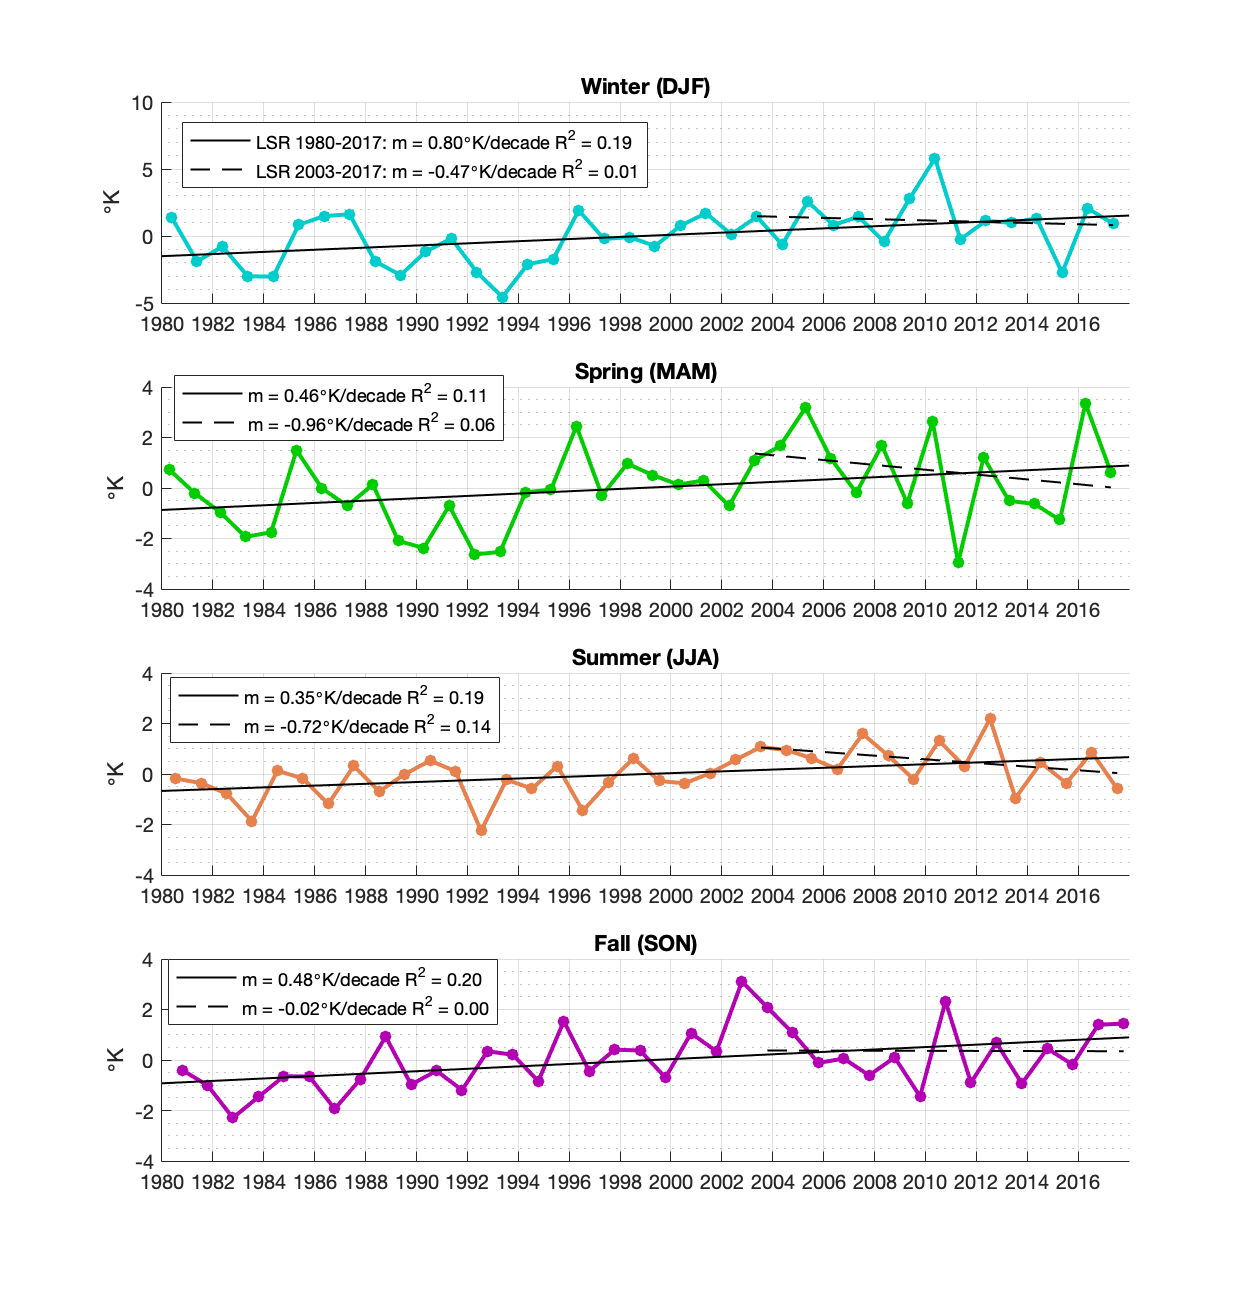
\includegraphics[width=0.9\textwidth]
{/Users/benjamingetraer/Documents/IndependentWork/senior-thesis/figures/spring2019/SeasonalTall.png}}
\caption[Seasonal 2m temperature trends over the Greenland Ice Sheet: 1980--2017]{Seasonal trends in MERRA-2 2m air temperature across the Greenland Ice Sheet for 1980--2017. Plotted points are the seasonal mean for each year, and are fit with a type-1 least squares regression for the full time period (solid) and the GRACE time period (dashes). Note that between 1980--2017 Winter temperatures warmed more than Summer temperatures, while during the GRACE time period (2003--2017) Summer temperatures dropped more than Winter temperatures. Table~\ref{tab:seasonaltrends} contains an analysis of the significance of each trend and its confidence interval, showing that the seasonal trends in mean monthly temperature over the full time period are significant, while the seasonal trends over the GRACE period are not significantly differentiable (in both $p$-value and confidence interval) from trends in random data drawn randomly from a similar normal distribution. \label{fig:seasonalclimate}}
\end{figure}
%%%%%%%%%%%%%%%%%%%%%%%%%%%%%%%%%%%%%%%%%%%%%%%%%%%%%%%%%%%%%%%%%%%%%%%%%%%%%%%%%%%%%%%%%%


%%%%%%%%%%%%%%%%%%%%%%%%%%%%%%%%%%%%%%%%%%%%%%%%%%%%%%%%%%%%%%%%%%%%%%%%%%%%%%%%%%%%%%%%%%
%	TSLOPES FIGURE
%%%%%%%%%%%%%%%%%%%%%%%%%%%%%%%%%%%%%%%%%%%%%%%%%%%%%%%%%%%%%%%%%%%%%%%%%%%%%%%%%%%%%%%%%%
 \begin{figure}[h]
\centering
\makebox[\linewidth][c]{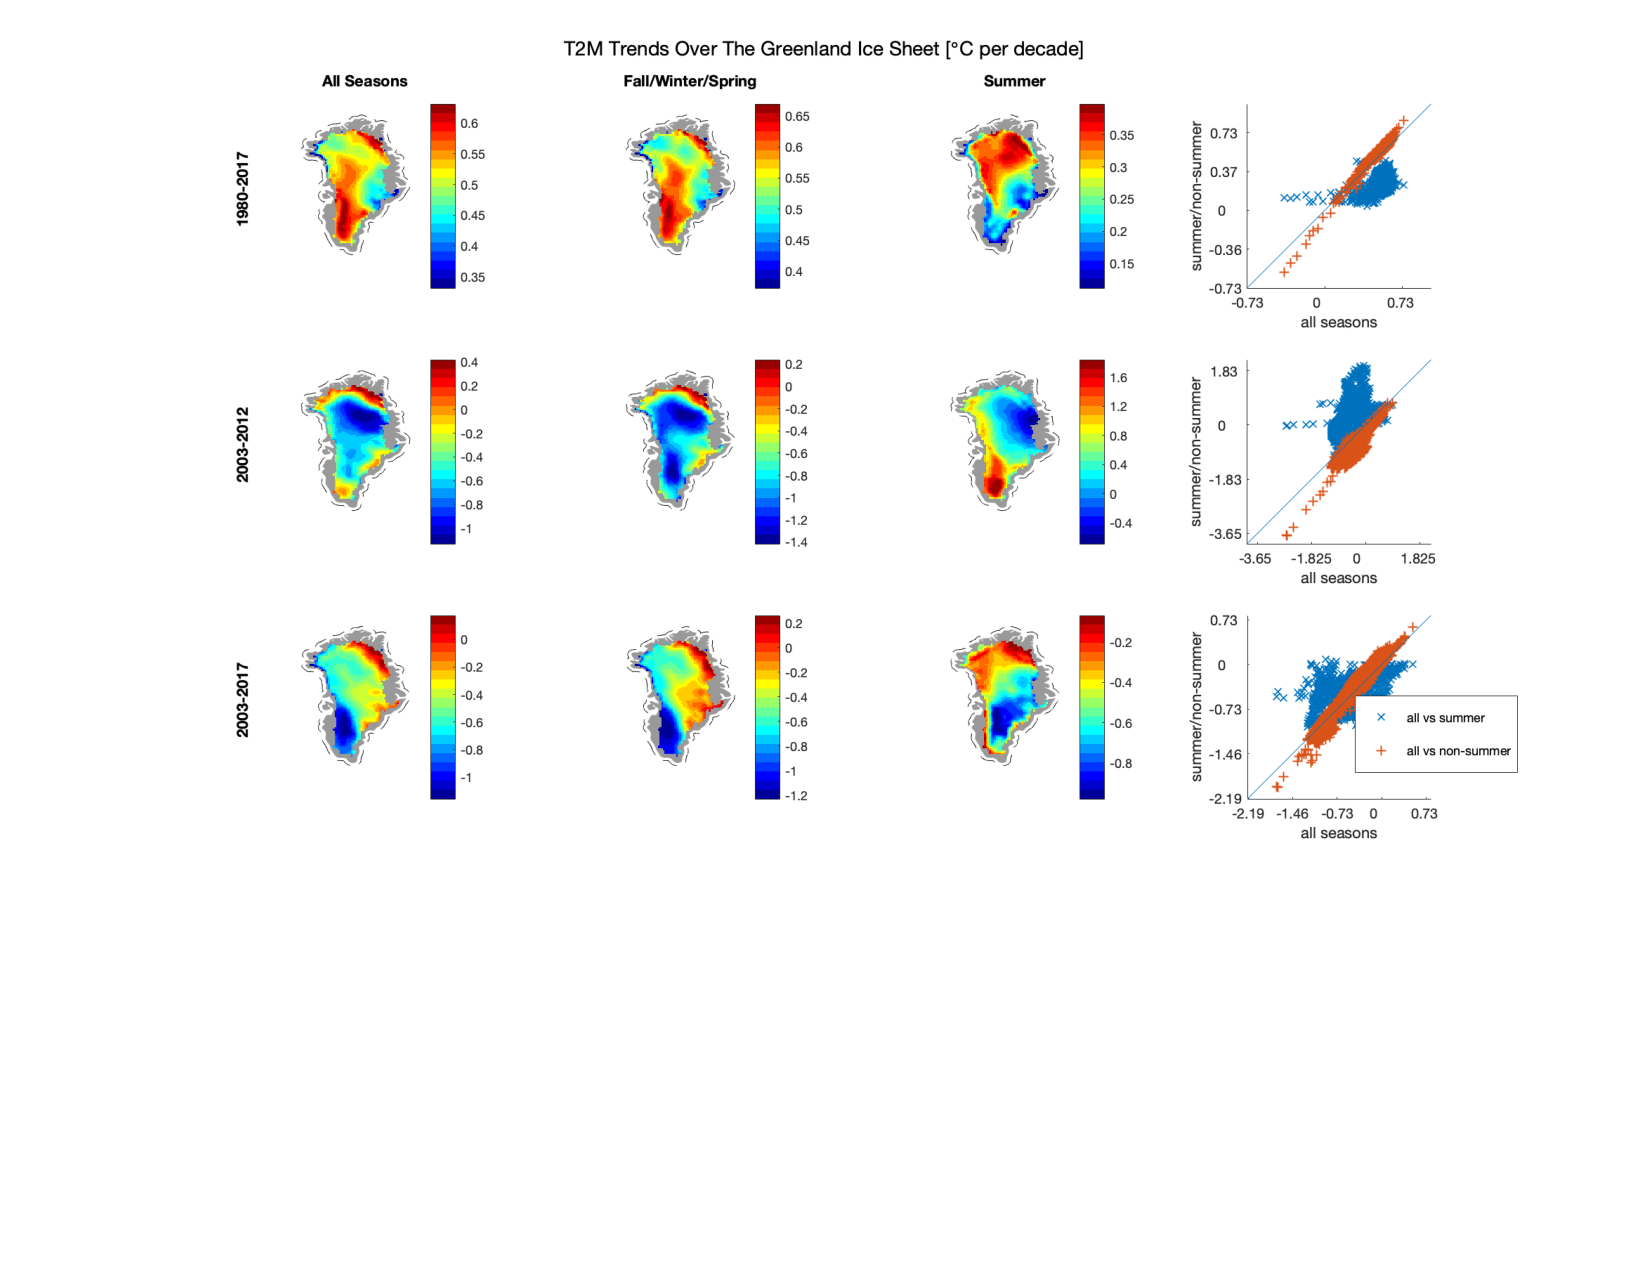
\includegraphics[width=1.2\linewidth]
{/Users/benjamingetraer/Documents/IndependentWork/senior-thesis/figures/spring2019/TempSlopes.pdf}}
\caption[Spatial Variability of Temperature Anomaly Trends]{Linear trends in near surface temperature anomaly across the Greenland Ice Sheet. The trend maps show three different time periods in separate rows, and three different seasonal combinations in separate columns. Note that over the entire 1980--2017 record, Summer warming has occurred mostly in the N and NW regions. In contrast to that 37 year trend, the first decade of GRACE saw concentrated Summer warming in the SW. This SW warming did not continue through the last 5 years of the time period, which saw a counter balancing cooling in the S and warming in the N, resulting in an apparent overall Summer cooling over the entire 2003--2017 time period. The crossplots in the righthand column show the strong correlation of non-Summer months to the trends seen when all seasons are considered, demonstrating that Summer trends are significantly different from the trends seen in other seasons, and are almost completely obscured unless Summer months are specifically isolated. Trend values are type-1 least square regressions after removing seasonal cycles.} \label{fig:tslopes}
\end{figure}
%%%%%%%%%%%%%%%%%%%%%%%%%%%%%%%%%%%%%%%%%%%%%%%%%%%%%%%%%%%%%%%%%%%%%%%%%%%%%%%%%%%%%%%%%%


%%%%%%%%%%%%%%%%%%%%%%%%%%%%%%%%%%%%%%%%%%%%%%%%%%%%%%%%%%%%%%%%%%%%%%%%%%%%%%%%%%%%%%%%%%%%%%%%%%%%%%%%%%%%%%%%%%%%%%%%%%%%%%%%%%%%%%%%%%%%%%%%%%%%%%%%%%%%%%%%%%%%%%%%%%%%%%%%%%%%
%% Warmest seasons
%%%%%%%%%%%%%%%%%%%%%%%%%%%%%%%%%%%%%%%%%%%%%%%%%%%%%%%%%%%%%%%%%%%%%%%%%%%%%%%%%%%%%%%%%%%%%%%%%%%%%%%%%%%%%%%%%%%%%%%%%%%%%%%%%%%%%%%%%%%%%%%%%%%%%%%%%%%%%%%%%%%%%%%%%%%%%%%%%%%%
\begin{table}[!h]
\begin{center}
\begin{tabular}{ |c|l|c||c|c|c| } 
\hline
 & \multicolumn{2}{c}{\bfseries{Summer (JJA)}} & \multicolumn{2}{c|}{\bfseries{Winter (DJF)}} \\
\hline
 & \bfseries{Year} & \bfseries{T2M anom. $^{\circ}$C} & \bfseries{Year} & \bfseries{T2M anom. $^{\circ}$C}\\
\hline
1	& 	2012 (1)	&	$2.19 \pm 0.51$ &	2010	&	$5.28  \pm 0.70$	\\
2	&   2007 (7)	&	$1.59 \pm 0.56$ &	1980	&	$3.23  \pm 2.19$	\\
3	&   2010 (3)	&	$1.32 \pm 0.77$ &	2011	&	$3.06  \pm 2.67$	\\
4	&   2003 (8)	&	$1.07 \pm 1.02$ &	2003	&	$2.75  \pm 1.59$	\\
5	&   2004 (13)	&	$0.95 \pm 0.55$ &	2007	&	$2.34  \pm 1.84$	\\
6	&   2016 (2) 	&	$0.86 \pm 0.50$ &	2013	&	$2.25  \pm 0.34$	\\
7	&   2008 (9)	&	$0.73 \pm 0.25$ &	1986	&	$1.75  \pm 2.92$	\\
8	&   1998 		&	$0.63 \pm 0.59$ &	2009	&	$1.70  \pm 0.48$	\\
9	&   2005 (5)	&	$0.62 \pm 1.22$ &	1996	&	$1.46  \pm 0.48$	\\
10	&   2002		&	$0.56 \pm 1.60$ &	1987	&	$2.35  \pm 3.79$	\\
\hline
\end{tabular}
\caption[Warmest seasons over Greenland Ice Sheet]{Top 5 years ranked by highest mean 2m air temperature for Summer and Winter seasons over the Greenland Ice Sheet (1980--2017). Adjacent to the year, in parentheses, is that year's rank by greatest mass loss (2003--2017). Mean temperature is the mean of the three monthly means in that season, and the reported error is the standard of deviation of the three monthly means in that season. Despite a downward drift in mean temperature between 2003--2017, a majority of the top ten warmest seasons on record occurred within that time frame. Note the separation of 2012 from the next closest years, making it the warmest Summer on record. Worth noting is that 2013, the year of least mass loss on the GRACE record, ranks as the 5th coldest Summer season in the 1980--2017 record, and the coldest Summer season of the GRACE time period. \label{tab:rankedseasons}}
\end{center}
\end{table}
%%%%%%%%%%%%%%%%%%%%%%%%%%%%%%%%%%%%%%%%%%%%%%%%%%%%%%%%%%%%%%%%%%%%%%%%%%%%%%%%%%%%%%%%%%%%%%%%%%%%%%%%%%%%%%%%%%%%%%%%%%%%%%%%%%%%%%%%%%%%%%%%%%%%%%%%%%%%%%%%%%%%%%%%%%%%%%%%%%%%




\clearpage
\subsection{Comparison of Mass Loss and MERRA-2 Variables}		

As a first order analysis of atmospheric drivers of ice loss, I compared the net change in Greenland mass over the entire GRACE period to mean the average Summer (JJA) surface skin temperature (ST), 2 meter air temperature (T2M), and 2 meter specific humidity (QV2M) over the entire period (Figure~\ref{fig:comparisontotal}). Point-to-point comparisons were binned every by mass loss, showing a positive correlation between temperature and humidity and ice loss, as generally expected (Figure~\ref{fig:comparisontotal}). 

For areas with less than $750$~kg/m$^2$ of ice loss over 2003--2017, higher amounts of ice loss correlated with quadratically higher temperatures and humidity (melting more ice requires a non-linear increase in temperature, Figure~\ref{fig:comparisontotal})). In contrast, there was no difference in mean temperature between areas with $750$~kg/m$^2$ of ice loss and those with $2000$~kg/m$^2$, and it was only at losses over $2750$~kg/m$^2$ at which mean temperature and humidity had to be significantly higher (Figure~\ref{fig:comparisontotal}). 

The plateau in the relationship between mean temperature and humidity and mass loss of $750$--$2500$~kg/m$^2$ (2003--2017) is the effect of GRACE detected mass loss within that range aligning with a large variance in mean temperature (Figure~\ref{fig:comparisontotal}). The average surface temperature (ST) within that range of mass loss hovers just above $-8.15^{\circ}$C ($265^{\circ}$K), corresponding generally with the mid-range of the ice sheet, below the upper accumulation zone where mass change was positive, but shy of the periphery (Figure~\ref{fig:comparisontotal}). Over the 2003--2017 record, mean ST was consistently about $2^{\circ}$C lower than T2M, and examining the best fit regressions between the two temperatures and the GRACE data, mass loss may to be subtly more sensitive to ST---melting more ice requires a smaller change in ST than T2M (Figure~\ref{fig:comparisontotal}).

Similar comparisons were conducted for each quadrant of Greenland comparing total mass loss to T2M (Figure~\ref{fig:comparisonregions}). The eastern half of the ice sheet showed strong quadratic correlation between mass loss and temperature for areas with less than $1000$~kg/m$^2$, and the correlation in the NE never plateaus (Figure~\ref{fig:comparisonregions}). In contrast, the quadratic relationship for the western half of the ice sheet extends only to areas of less than $750$~kg/m$^2$ in the NW, and barely exists in the SW where a subregion estimated by GRACE to have near $0$~kg/m$^2$ of mass loss is located in one of the highest temperature coastal environments on the ice sheet (Figure~\ref{fig:comparisonregions}). 



%%%%%%%%%%%%%%%%%%%%%%%%%%%%%%%%%%%%%%%%%%%%%%%%%%%%%%%%%%%%%%%%%%%%%%%%%%%%%%%%%%%%%%%%%%
%	2003--2017 MASS vs Mean Climate variables %%%%%%%%%%%%%%%%%%%%%%%%%%%%%%%%%%%%%%%%%%%%%%%%%%%%%%%%%%%%%%%%%%%%%%%%%%%%%%%%%%%%%%%%%%
 \begin{figure}[h]
\centering
\makebox[\linewidth][c]{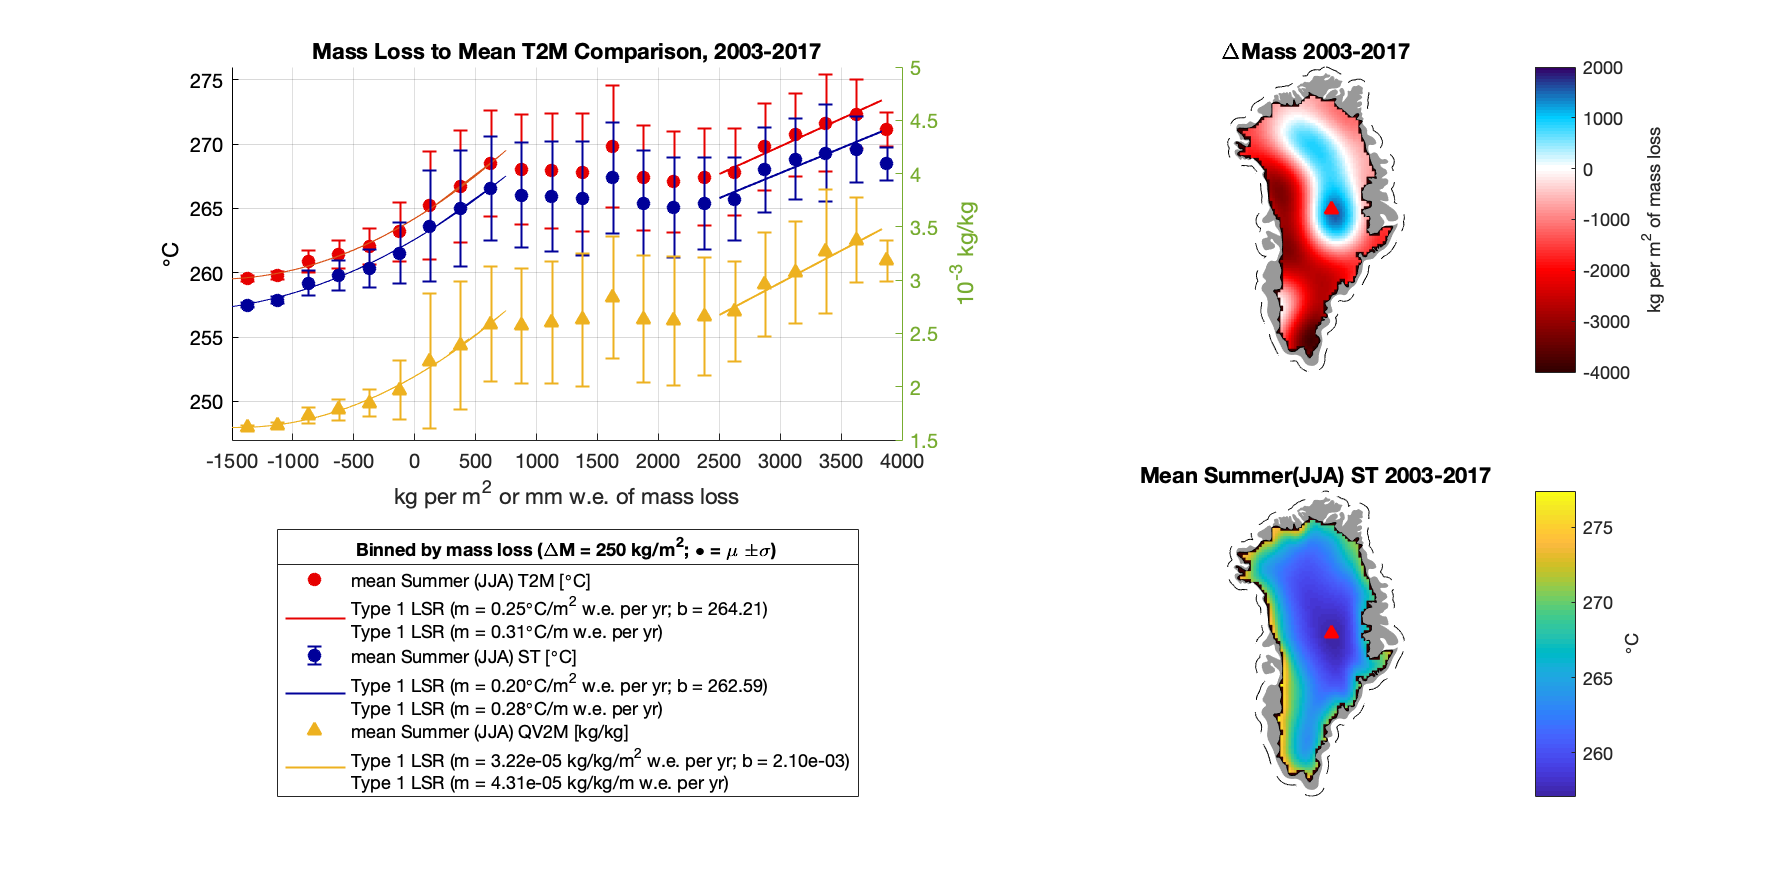
\includegraphics[width=1.2\linewidth]
{/Users/benjamingetraer/Documents/IndependentWork/senior-thesis/figures/spring2019/TotalMassLossComparison.png}}
\caption[Comparison of Total Mass Loss with T2M, ST, QV2M: 2003--2012]{Total mass change over the Greenland Ice Sheet, compared to the average daily mean near-surface temperature (T2M,~red), skin surface temperature (ST,~blue), and near surface specific humidiy (QV2M,~yellow) for the June/July/August Summer season. MERRA-2 data were smoothed using Matlab's gaussian smoothing filter and a smoothing kernel of $\sigma=1\mathrm{std}$ before being bi-linearly interpolated on the grid (see Figure~\ref{fig:gridbasins}). Cross-plotted data were binned every $250$~kg/m$^2$, with the mean and standard of deviation are represented here. Note that in zones of mass accumulation (negative mass loss on the $x$-axis) and loss of $750$~kg/m$^2$ (or mm of water equivalence, mm w.e.) average temperatures and humidity over 2003--2017 scales quadratically with increasing mass loss, while regions with $750$--$2500$~kg/m$^2$ of loss have similar ranges, and regions with $>2500$~kg/m$^2$ of loss seem to scale linearly. The quadratic and linear relationships are shown in the legend in two lines, the first giving the acceleration and intercept of the modeled variable per $1000$~kg/m$^2$ (m$^2$~w.e.) for mass loss $<750$~kg/m$^2$, and the second giving the linear rate of the modeled variable per $1000$~kg/m (m~w.e.). As the mass losses are for the entire 14 year GRACE record, these rates were normalized to reflect the amount of ice loss per year that a given change in the modeled variable relates to.
\label{fig:comparisontotal}}
\end{figure}
%%%%%%%%%%%%%%%%%%%%%%%%%%%%%%%%%%%%%%%%%%%%%%%%%%%%%%%%%%%%%%%%%%%%%%%%%%%%%%%%%%%%%%%%%%		


%%%%%%%%%%%%%%%%%%%%%%%%%%%%%%%%%%%%%%%%%%%%%%%%%%%%%%%%%%%%%%%%%%%%%%%%%%%%%%%%%%%%%%%%%%
%	2003--2017 MASS vs Mean Climate variables %%%%%%%%%%%%%%%%%%%%%%%%%%%%%%%%%%%%%%%%%%%%%%%%%%%%%%%%%%%%%%%%%%%%%%%%%%%%%%%%%%%%%%%%%%
 \begin{figure}[h]
\centering
\makebox[\linewidth][c]{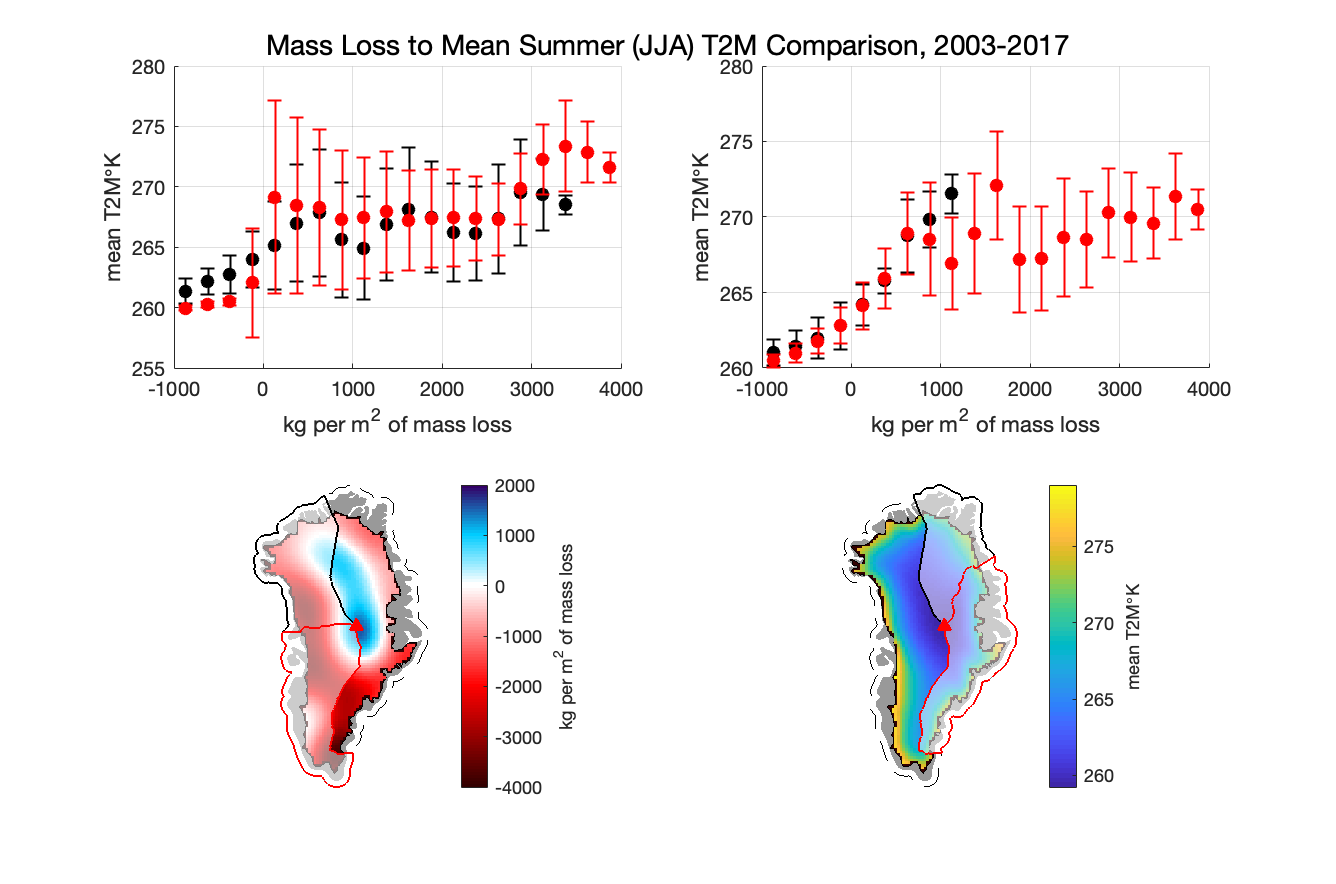
\includegraphics[width=1.2\linewidth]
{/Users/benjamingetraer/Documents/IndependentWork/senior-thesis/figures/spring2019/RegionalMassLossComparison.png}}
\caption[Comparison of Regional Mass Loss with T2M: 2003--2012]{Total mass change over the Greenland Ice Sheet, compared to the average daily mean near-surface temperature (T2M,~red), and divided by region (see Figure~\ref{fig:comparisontotal} for method details, and Figure~\ref{fig:gridbasins} for regional definitions). The eastern (western) regions are shown to the left (right), with N and S quadrants outlined in black and red respectively at the bottom, corresponding to the black and red binned scatter plots above. Note that the NE shows the most coherent quadratic relationship between mass loss and T2M, and also has the lowest amounts of mass loss. In contrast, the SW has a wide range of mass loss and an area of low mass loss along the coast which disrupts the relationship bewteen T2M and mass.} \label{fig:comparisonregions}
\end{figure}
%%%%%%%%%%%%%%%%%%%%%%%%%%%%%%%%%%%%%%%%%%%%%%%%%%%%%%%%%%%%%%%%%%%%%%%%%%%%%%%%%%%%%%%%%%		



%%%%%%%%%%%%%%%%%%%%%%%%%%%%%%%%%%%%%%%%%%%%%%%%%%%%%%%%%%%%%%%%%%%%%%%%%%%%%%%%%%%%%%%%%%
%	2003--2012 TEMP and MASS trends
%%%%%%%%%%%%%%%%%%%%%%%%%%%%%%%%%%%%%%%%%%%%%%%%%%%%%%%%%%%%%%%%%%%%%%%%%%%%%%%%%%%%%%%%%%
 \begin{figure}[h]
\centering
\makebox[\linewidth][c]{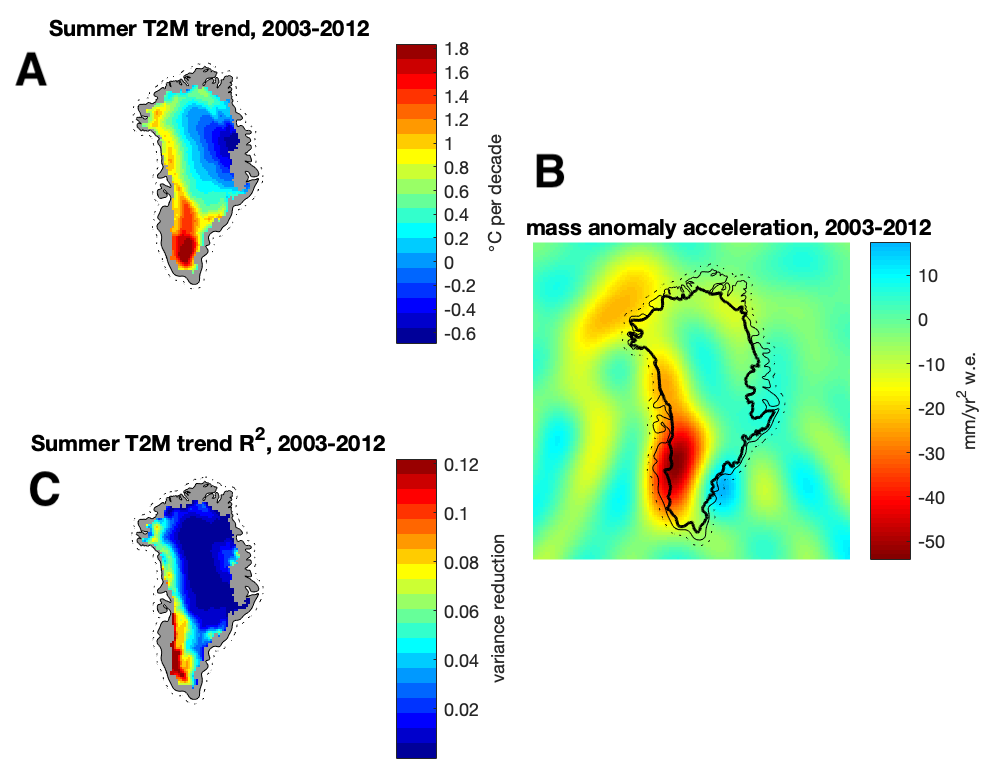
\includegraphics[width=1.2\linewidth]
{/Users/benjamingetraer/Documents/IndependentWork/senior-thesis/figures/spring2019/TempMassTrend2.png}}
\caption[Near Surface Temperature and Mass Anomaly Trends: 2003--2012]{Near surface temperature trend (\textbf{A}), and mass anomaly acceleration (\textbf{B}), between 2003--2012 (see Figure~\ref{fig:tslopes}). Note the positive temperature trend in the SW coincident with increasing rates of mass loss over that time period. The quality of fit for the temperature trend is shown in (\textbf{C}). Note that the strongest correlation occurs along the coast, also in very similar orientation to the GRACE signal.
} \label{fig:tslopesSummer}
\end{figure}
%%%%%%%%%%%%%%%%%%%%%%%%%%%%%%%%%%%%%%%%%%%%%%%%%%%%%%%%%%%%%%%%%%%%%%%%%%%%%%%%%%%%%%%%%%













\clearpage
%%%%%%%%%%%%%%%%%%%%%%%%%%%%%%%%%%%%%%%%%%%%%%%%%%%%%%%%%%%%%%%%%%%%%%%%%%%%%%%%%%%%%%%%%%
%%%%%%%%%%%%%%%%%%%%%%%%%%%%%%%%%%%%%%%%%%%%%%%%%%%%%%%%%%%%%%%%%%%%%%%%%%%%%%%%%%%%%%%%%%
%	DISCUSSION
%%%%%%%%%%%%%%%%%%%%%%%%%%%%%%%%%%%%%%%%%%%%%%%%%%%%%%%%%%%%%%%%%%%%%%%%%%%%%%%%%%%%%%%%%%
%%%%%%%%%%%%%%%%%%%%%%%%%%%%%%%%%%%%%%%%%%%%%%%%%%%%%%%%%%%%%%%%%%%%%%%%%%%%%%%%%%%%%%%%%%
\section{Discussion}


%%%%%%%%%%%%%%%%%%%%%%%%%%%%%%%%%%%%%%%%%%%%%%%%%%%%%%%%%%%%%%%%%%%%%%%%%%%%%%%%%%%%%%%%%%
%	OVERALL TEMP
%%%%%%%%%%%%%%%%%%%%%%%%%%%%%%%%%%%%%%%%%%%%%%%%%%%%%%%%%%%%%%%%%%%%%%%%%%%%%%%%%%%%%%%%%%
Analysis of near surface temperature indicates that the warming of the 1990's brought average temperatures on the ice sheet to a level that remained significantly higher than previous decades, despite downward drift through the GRACE time period (see Figure~\ref{fig:climatewarming}). Leading into the first years of the GRACE record, average near surface Summer temperatures on ice sheet as a whole were $\sim0.8^{\circ}$C warmer than at the beginning of the 1980's (Figure~\ref{fig:seasonalclimate}), and through the first decade of GRACE (2003--2012), warming Summer temperature trends focused in the SW region estimate an additional increase in Summer temperatures of $0.8$--$1.8^{\circ}$C (Figure~\ref{fig:tslopes}). These estimations of a temperature anomaly of almost $3^{\circ}$C in the SW in 2012 (compared to temperatures of the early 1980's) are similar to estimates which put the Summer of 2012 at $4^{\circ}$C warmer than the 1960--1990 average \cite[][]{angelen2014}.



%%%%%%%%%%%%%%%%%%%%%%%%%%%%%%%%%%%%%%%%%%%%%%%%%%%%%%%%%%%%%%%%%%%%%%%%%%%%%%%%%%%%%%%%%%
%	TEMP MASS RELATIONSHIP
%%%%%%%%%%%%%%%%%%%%%%%%%%%%%%%%%%%%%%%%%%%%%%%%%%%%%%%%%%%%%%%%%%%%%%%%%%%%%%%%%%%%%%%%%%
\subsection{Comparing GRACE ice loss to temperature}
Assuming that the physical relationship between temperature and melt is the same across the ice sheet, the underlying cause of the plateau in Figure~\ref{fig:comparisontotal} may be related to measurement, interannual variability, or mass movement. Bias and spatial resolution in GRACE continues to be pushed \cite[see][]{Harig+2012,save2016,getraerSpring}, but remains conservatively estimated at $\sim300$km $\times$ $300$km \cite[][; Greenland itself is approximately $2700$km North--South $\times$ $1200$km East--West]{scanlon2016}. 

Regions between the strong mass loss of the lower ice sheet and mass gain in the accumulation zone may be poorly resolved, and not accurately reflect local melt. This explanation is directly supported by the clear positive correlation between temperature, humidity, and mass loss seen at both the positive and negative extremes of mass anomaly, suggesting that the spherical harmonic basis of the GRACE data captures peaks of mass anomaly even when they are relatively close together (Figure~\ref{fig:comparisontotal}). Mass loss extremes on Greenland are located just over $400$km away from each other, nearing the limit of GRACE resolution, and transitions between those areas may be biased by those extremes.

Complicating the spatial limitations of GRACE are the dimensions of the ice sheet itself. The steeper eastern slopes of the ice sheet have less melt for a given temperature anomaly, simply due to the distribution of the low altitude ablation zone in those regions \cite[][]{bevis2019}. As a result, the short-distance gradient in mass anomaly captured by GRACE is not as extreme on the eastern half of the ice sheet as it is on the western half, where a larger distribution of low altitude ice in the ablation zone is exposed temperature fluctuations. If GRACE may struggle to accurately resolve regions which fall in between very close extrema of mass anomaly (distances which approach the satellites' fundamental spatial resolution), we would expect the NE quadrant to have the clearest spatial correlation with temperature, which we do in fact observe (Figure~\ref{fig:comparisonregions}).

Another factor at play in the connection between total mass lost and mean temperature over a 14 year period is inter-annual variability. Taking a mean temperature over such a timescale obscures short periods of intense melting, which may have a significant contribution to total melt.

Additionally, while temperature and humidity contribute to melting ice, the redistribution of mass after ice is melted can differ depending on local conditions, and may flow relatively directly off of the ice sheet, or get stored within the snowpack or refrozen, conditions which themselves have changed dramatically over the GRACE observation period \cite[][]{angelen2014,pena2015}.

\subsection{Concentration of melt in the SW}

The change in temperature anomaly tendency in the years just before and after 2012 aligns with similar patterns seen observed in atmospheric river tendencies, which focused more on the SW region prior to 2012, and more on the northern regions in following years \cite[][]{mattingly2018}. While it is unsurprising that warm air and moist air go hand in hand, a similar pattern in net short-wave radiation and microwave-derived melt days was also observed in the years leading up to 2012 \cite[][]{angelen2014}. The connection between air temperature, moisture, and radiation balance suggests that warm, moist air may enhance insolation driven melt not only by raising the baseline temperature of the ice surface, but by changing surface albedo and allowing greater absorption of insolation as suggested by \cite[][]{box2012}.
%
%%% WHAT FACTORS AFFECT??
%"Greenland Ice Sheet Surface Melt and Its Relation to Daily Atmospheric Conditions"

%% is Greenland warming?


%%%%%%%%%%%%%%%%%%%%%%%%%%%%%%%%%%%%%%%%%%%%%%%%%%%%%%%%%%%%%%%%%%%%%%%%%%%%%%%%%%%%%%%%%%
%	CONCLUSION
%%%%%%%%%%%%%%%%%%%%%%%%%%%%%%%%%%%%%%%%%%%%%%%%%%%%%%%%%%%%%%%%%%%%%%%%%%%%%%%%%%%%%%%%%%
\section{Conclusion}
The melting of the Greenland Ice Sheet is strongly connected to warming temperatures in much of the literature, and the significant repercussions of various short-term warming scenarios on the evolution of ice sheet melting are of great importance to predicting sea-level rise over the next century \cite[][]{hahn2018,pattyn2018,ruckamp2018}. To best understand the relationship between warming temperatures and Greenland melt, some caution must be used in drawing a direct line between increasing mean global surface temperatures and increases of melt on the Greenland Ice Sheet, as temperature on the Greenland Ice Sheet has not risen in the same pattern as the broader Northern Hemisphere (see Figure~\ref{fig:climatewarming}. 

Between the late 1990's and 2012, an apparent pause in the rise of mean global temperatures coincided with the strongest acceleration in Greenland Ice Sheet mass loss of the last century, a ``hiatus'' observed in global warming over the first decade of the 21st century that has been correlated with natural climate variability such as the El Ni\~{n}o/Southern Oscillation \cite[][]{kosaka2013,angelen2014,bevis2019}. Between 2012 and 2017, mean global temperatures resumed a strong upwards trend driven by a negative to positive shift in ENSO phase.

%\begin{figure}[h]
%\centering
%\makebox[\textwidth][c]{\includegraphics[height=0.5\textheight]
%{/Users/benjamingetraer/Documents/IndependentWork/senior-thesis/figures/spring2019/ENSO_TEMP.png}}
%\caption[]{} \label{fig:ENSO}
%\end{figure}

Over the same period, mean Greenland Ice Sheet near-surface temperature did not rise significantly, and in fact was decreasing slightly on average between 2003 and 2017 \cite[see Figs.~\ref{fig:seasonalclimate}~\&~\ref{fig:tslopes}, and ][]{hearty2018, westergaard2018,reeves2017}. Mean temperatures over Greenland are expected to continue to rise with global temperatures into the future, but have not done so significantly since the 1990's \cite[][]{reeves2017}, even with the return of Northern Hemisphere warming.

In interpreting the record of Greenland Ice Sheet mass wasting, it is important to note that the linear trend observed over the entire 2003--2017 GRACE record (Figure~\ref{fig:Getraer}~B) need not be driven by changing climate over that time period. Warming mean temperatures over Greenland in the 1990's drove the ice sheet into the linear decline we have seen in the GRACE record, with an approximately constant amount of Summer loss each year \cite[][]{getraerFall}. Over that time period, anomalous years and temporary increased rates in melt are explained by variability in weather patterns across Greenland and the North Atlantic, including temporary regional warming trends \cite[see Figure~\ref{fig:tslopesSummer}][]{bevis2019,hahn2018}. It would appear that Greenland ice loss may remain in linear decline affected by natural variability until a period of sustained significant warming occurs, such as was seen in the 1990's.




%\begin{figure}[h]
%\centering
%\makebox[\textwidth][c]{\includegraphics[height=0.5\textheight]
%{/Users/benjamingetraer/Documents/IndependentWork/senior-thesis/figures/spring2019/Tslope.png}}
%\caption[]{} \label{fig:Tslope}
%\end{figure}
%
%% using the NAO
%\subsection{NAO Correlation with Melt}
%Often times when comparing the NAO to Greenland melt, monthly or seasonal means are used to correlate with melt events that occur over time scales of a few days \cite[see, for example, ][]{mattingly2018, bevis2019, angelen2014}. These averaged NAO index values are used despite the fact that daily and sub-daily solutions are readily available for the NAO index, and despite the fact that the physical atmospheric drivers of melting (such as temperature, cloud cover, etc.) are changing on a daily, not monthly, basis, and are interacting directly with atmospheric pressure \cite[for example,][]{mattingly2018}. 



\clearpage

% APPENDIX A --- DATA SOURCES
\newpage 
\appendix

\section{Appendix A: Data and code sources \label{app:a}}

\textit{RL05 spherical harmonic coefficients for the time-variant geopotential field from the Center for Space Research data processing center at The University of Texas at Austin are available at:} \\
\indent \url{ftp://podaac.jpl.nasa.gov/allData/grace/L2/CSR/RL05}\\

\noindent\textit{Coefficients describing Earth's center of mass \cite[spherical harmonic degree~1, from][]{swenson2008} are available at:} \\
\indent\url{ftp://podaac-ftp.jpl.nasa.gov/GeodeticsGravity/tellus/L2/degree_1/}\\

\noindent\textit{Coefficients describing Earth's oblateness \cite[spherical harmonic degree~2, order~0, from][]{cheng2013} are available at:} \\
\indent \url{ftp://ftp.csr.utexas.edu/pub/slr/degree_2/}\\

\noindent\textit{Index values for the North Atlantic Oscillation are calculated by the National Weather Service Climate Prediction Center \cite[see][]{cpcNAO}, with normalized monthly average values since January 1950 available at:} \\
\indent \url{ftp://ftp.cpc.ncep.noaa.gov/wd52dg/data/indices/nao\_index.tim}\\
\indent\textit{Normalized daily values since January 1950 are available at:} \\
\indent \url{ftp://ftp.cpc.ncep.noaa.gov/cwlinks/norm.daily.nao.index.b500101.current.ascii}\\


\noindent\textit{MERRA-2 atmospheric reanalysis data are calculated by the NASA Global Modeling and Assimilation Office (GMAO) as part of the activities of NASA's Science Mission Directorate, and are archived and distributed by the Goddard Earth Sciences Data and Information Services Center (GES-DISC). All data was accessed between September 2018 and April 2019.} \\ 
\indent \textit{A graphical user interface for generating data download links for specific subsets of variables, space, and time is available at:} \url{https://disc.gsfc.nasa.gov}\\
\indent \textit{Data used in this study can be directly accessed at the following addresses:} \\
\indent \url{https://goldsmr4.gesdisc.eosdis.nasa.gov/data/MERRA2_MONTHLY/M2SMNXSLV.5.12.4/}\\
\indent \url{https://goldsmr4.gesdisc.eosdis.nasa.gov/data/MERRA2/M2T1NXSLV.5.12.4/}\\
\indent \url{https://goldsmr4.gesdisc.eosdis.nasa.gov/data/MERRA2/M2T1NXRAD.5.12.4/}\\


\noindent\textit{Northern Hemisphere Land-Ocean Temperature Index anomalies from NASA's Goddard Institute for Space Studies Surface Temperature Analysis \cite[GISTEMP v3, see][]{hansen2010} were accessed in March 2019 and are available at:} \\ 
\indent \url{https://data.giss.nasa.gov/gistemp/tabledata_v3/NH.Ts+dSST.csv}\\



\noindent\textit{MATLAB code for the expansion and manipulation of spherical harmonic
eigenfunctions into Slepian bases and manipulation of GRACE files is borrowed and adapted from:} \\
\indent \url{https://github.com/csdms-contrib/}\\

\noindent\textit{MATLAB code developed for this project, including functions for executing the wavelet analysis and scripts for generating figures, can be accessed at:} \\
\indent \url{https://github.com/bgetraer/slepian_bgetraer/}\\




%\noindent\textit{Outline coordinates for the Greenland ice scheet drainage basins from \cite{zwally} available at:}\\
%\indent \url{http://icesat4.gsfc.nasa.gov/cryo_data/ant_grn_drainage_systems.php}\\

\clearpage

% APPENDIX B
\newpage
\appendix

\section{Appendix B: GRACE methods of data reduction \label{app:b}}
\textbf{\textit{Adapted directly from} \textsc{Resolving and Contextualizing the Signal of Greenland Ice Loss 2014--2017}, \cite{getraerFall}, and \textsc{Regional Forcing of Greenland Ice Loss 2002--2017}, \cite{getraerSpring}}

{\it
The Gravity Recovery and Climate Experiment is a twin-satellite mission active
2002--2017, with its final data collection completed in October 2017. GRACE
measurements are made accessible in the form of several data products offered
through NASA and partnered agencies, which generally rely on a method of data
reduction to translate the ``Level~1'' GRACE measurements of satellite positions into globally projected mass anomaly estimations. There are two primary
methods of data reduction: The creation of ``mascons,'' roughly equal-area
sections around the globe on the scale of single arc-degrees, each assigned a
single number representing mass change, and the calculation of spherical
harmonic coefficients, which correspond to continuous functions in three
dimensions that when summed can model the spatially continuous variation of mass
on the surface of Earth. The difference between continuous and discrete data reduction (harmonics vs. mascons) often has to do with localization of the signal in time and space. Discrete solutions may not be able to ``see'' continuous large scale patterns, while continuous solutions necessarily ``hide'' information about very localized signals in a collection of globally continuous patterns.

The spherical harmonic method requires continuous functions on Earth's surface, whereby a field of interest can be developed into a series solution of
eigenfunctions $Y_{lm}(\theta,\phi)$, where $l$ refers to the ``order''
(integers $0$ to $\infty$) and $m$ the ``degree'' (integers $-l$ to $+l$) of
each harmonic ($\theta$ and $\phi$ reference location on the surface of Earth). Due
to limitations in computational power and in the spatial resolution of the data
being modeled by the harmonic functions, calculated solutions are bandlimited,
meaning that they are calculated up to a finite order $L$. See
\cite{Simons+2006a}, their section~3 for a concise summary. See our
Figure~\ref{fig:SlepvSH} for illustrations of low-order spherical harmonic
eigenfunctions.

\begin{figure}[h!]
\centering
\textbf{Comparison of Spherical Harmonic Eigenfunctions to Slepian Basis Eigentapers}\par\medskip
\includegraphics[height=0.5\textheight]
{/Users/benjamingetraer/Documents/IndependentWork/JuniorPaper/JP02/Figures/SlepvSH.pdf}
\caption[Comparison of Spherical Harmonic Eigenfunctions to Slepian Basis Eigentapers]{Three low-order spherical harmonic eigenfunctions $Y_{lm}(\theta,\phi)$ are illustrated in \textbf{A} as examples of the basic forms these functions take: zonal (left, $m=0$), sectoral (middle, $m=l$), and tesseral (right, $m\neq l\neq 0$). When expanded into a geographically-localized Slepian basis, the forms of these eigenfunctions have parallel eigentapers as illustrated in rows \textbf{B} and \textbf{C}. The eigentapers allow for reconstruction of a signal with power concentrated within a geographical basis, minimizing the effect of the signal outside of the basis on the series solution. $r$ is radius, $L$ is the bandlimit of maximum order $l$ used in the Slepian expansion.} \label{fig:SlepvSH}
\end{figure}

Monthly coefficients for bandlimited global spherical harmonic solutions of the
time-variable geopotential field are independently calculated by three different
processing centers (GFZ in Potsdam, Germany; CSR at University of Texas, Austin; JPL at
California Institute of Technology) and published publicly as the GRACE
Level~2 Release~05 products for a few different bandwidths (see
\nameref{app:a}). The RL05 product is pre-corrected to remove the time-invariant
geopotential field using the GRACE Gravity Model~03 \cite[][]{GGM032007}, and we
use coefficients describing Earth's center of mass \cite[spherical harmonic
degree~1, from][]{swenson2008} and oblateness \cite[spherical harmonic degree~2,
order~0, from][]{cheng2013} calculated from Satellite Laser Ranging in order to
accurately capture mass variations on scales much larger than the area covered
by the GRACE satellites (see \nameref{app:a}). The coefficients are released as contributions to gravitational potential in units of $\frac{kg^{2}}{s^{2}}$, and are converted to equivalent surface density on Earth in units of $\frac{kg}{m^{2}}$ using the method of \cite{wahr1998}. Mass estimates are calculated through area-integration, and converted to sea-level equivalence using the method of \cite{tian2015}.

A third method of data reduction uses the spherical harmonic coefficients in a linear combination of their respective functions to
constrain explanatory power to an arbitrary geographic location \cite[][]{Simons+2006a}.
This method generates linear combinations of the spherical harmonic
eigenfunctions $Y_{lm}(\theta,\phi)$ called scalar Slepian functions
$g_{\alpha}(\theta,\phi)$, where $\alpha$ refers to the ``rank'' of the Slepian
function, which is a single linear combination of all spherical harmonic
eigenfunctions up to order $L$, also referred to as an ``eigentaper.'' Formally, this expansion is expressed in terms of the spherical harmonic eigenfunctions by:
\begin{equation}\label{eq:sh}
\sum_{l=0}^{L}\sum_{m=-l}^{l}f_{lm}Y_{lm}(\theta,\phi)= 
\sum_{\alpha=1}^{(L+1)^{2}}f_{\alpha}g_{\alpha}(\theta,\phi)
\end{equation}
	By construction the functions $g_{\alpha}(\theta,\phi)$ are centered around the geographic region of interest. A few eigentapers are concentrated in power strictly within the region, and most are concentrated in power predominantly outside of the region. The signal within the region is approximated by choosing those functions $g_{\alpha}(\theta,\phi)$ whose ratio of power inside of that region to outside of the region is significant (often around $\geq\frac{1}{2}$), the number of which is referred to as the Shannon number $N$. The resulting spatially concentrated estimation of the global field is expressed in the approximation:
\begin{equation}\label{eq:sh2sf}
\sum_{l=0}^{L}\sum_{m=-l}^{l}f_{lm}Y_{lm}(\theta,\phi)\approx 
\sum_{\alpha=1}^{N}f_{\alpha}g_{\alpha}(\theta,\phi)
\end{equation}
Though limited by $N$, the Slepian expansion is useful by reducing the
unnecessary information in the global spherical harmonic coefficients --- namely,
the signal everywhere else in the world. The method of calculating
geographically constrained scalar Slepian functions from a bandlimited series of
spherical harmonics, as well as the relationship between the geographical area
and the Shannon number is described in mathematical detail by
\cite{Simons+2006a}. See our Figure~\ref{fig:SlepvSH} for illustrations of low-rank
Slepian eigentapers in an circular, axisymmetric basis and a Greenland basis.

Slepian-based harmonics have the advantage of continuous solutions as opposed to
the coarse rasterized solutions of mascons, with less of the noise and bias
associated with globally continuous spherical harmonics. The expansion of global
spherical harmonics into a localized Slepian basis of eigentapers allows for
locally constrained signals to be extracted from the continuous global GRACE
RL05 data product with less impact from noise or signals from other geographic
locations, a problem that reduces the precision of the standard spherical
harmonic method. We will find localized mass anomaly solutions using the Slepian
expansion method of data reduction from the GRACE CSR
RL05 $L=60$ spherical harmonic coefficients \citep[see][]{Harig+2012}.


%\begin{wrapfigure}{r}{0.5\textwidth} 
\begin{figure}
\centering
\makebox[\textwidth][c]{
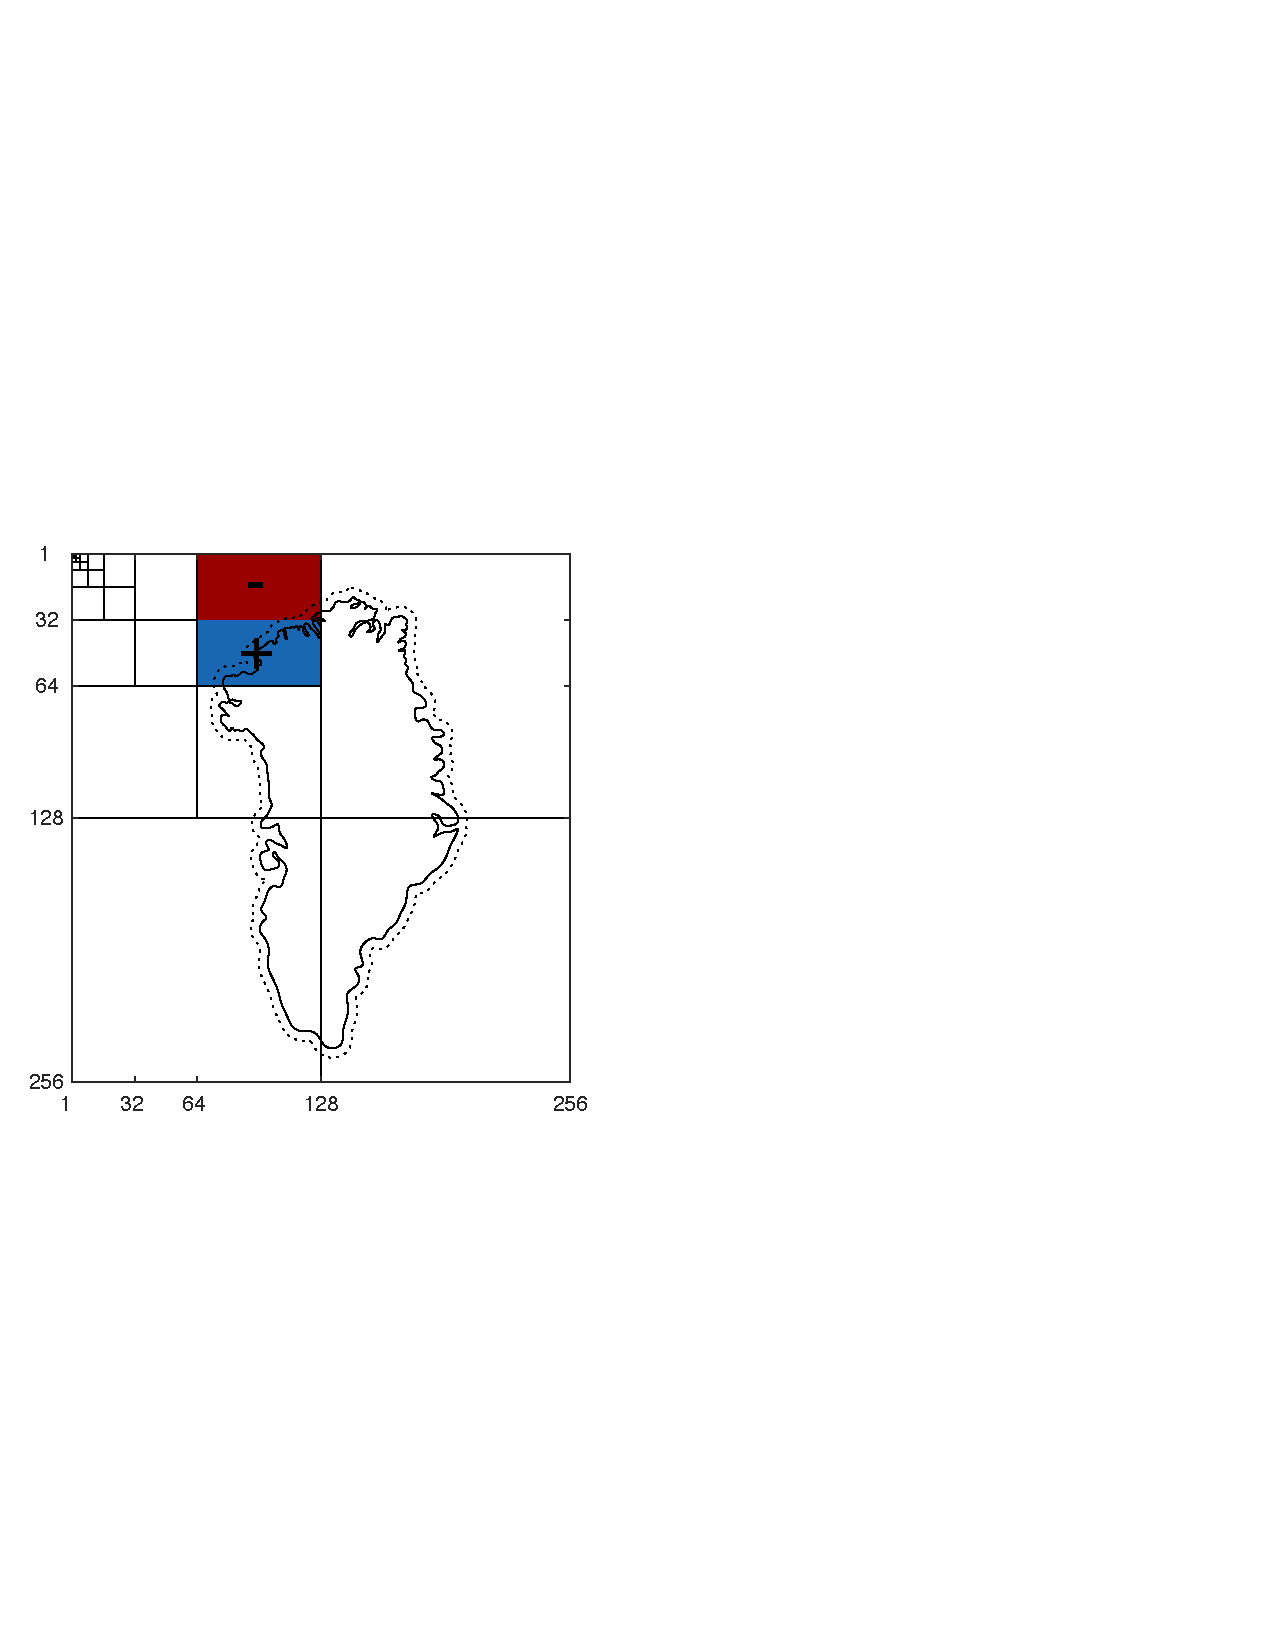
\includegraphics[width=0.5\linewidth]{/Users/benjamingetraer/Documents/IndependentWork/senior-thesis/figures/spring2019/wavemodel.pdf}}
\caption[The Wavelet Grid Around Greenland]{The grid extent around Greenland is defined in the global basis on a face of the \textit{Cubed Sphere} centered on Greenland \cite[see Figure~\ref{fig:gridbasins}~\textbf{A}~\&][]{ronchi1996}. In the image basis the grid is cartesian with length $256$. Grid lines in the image basis represent the diminishing areal support of wavelets of different levels, from $\zeta=8$ (the entire image) to $\zeta=1$ (a unit grid cell). Note that in reality, each wavelet level has coverage over the entire image. An example of a Haar wavelet basis function with discrete spatial support is shown in color. The dotted line around Greenland is a coastal buffer of $0.5^{\circ}$ as in Figure~\ref{fig:Getraer}~\& \cite{Harig+2016}.} \label{fig:thegrid}
%\end{wrapfigure}
\end{figure}

A fourth method of data reduction was explored in \cite{getraerSpring}, using 2-dimensional wavelet decomposition to define the spatial scales at which significant changes in mass loss were occurring in a specific area over a specific time-scale. Wavelets are oscillating functions with finite support in space. Wavelets of different scales capture signal at different resolution levels, and a discrete implementation of the transform would subsample a spatial grid depending on the scale. Each wavelet at each grid scale is assigned a weighting coefficient such that signal information at a location on the grid can be represented as a superposition of individual wavelets at different scale levels at that point. The weighting $m_{\beta}$ associated with the wavelet $w_{\beta}$ at each grid point, and at different scales of resolution, tells us where and how important information is at different scales (see Table~\ref{tab:exp_eq}~\& Figure~\ref{fig:thegrid}).



\begin{table}
\centering
\begin{tabular}{lll}
Approximation method & Expansion Equations & Spatial Support \\
\hline
Spherical Harmonic &  $\begin{aligned} M_{SH}(\underline{r}) = \sum_{l=0}^{L} \sum_{m=-l}^{+l} f_{lm} Y_{lm}(\underline{r}) \end{aligned}$ & global
\\
Slepian Functions & $\begin{aligned} M_{SF}(\underline{r}) = \sum_{\alpha=1}^{N} f_{\alpha} g_{\alpha}(\underline{r}) \end{aligned}$ & concentrated
\\
Wavelet Basis &  $\begin{aligned} M_{WB}(\underline{r}) = \sum_{\beta=1}^{K} m_{\beta} w_{\beta}(\underline{r}) \end{aligned}$ & compact
\end{tabular}
\caption[Expansion Equations for GRACE Data]{Expansions used to represent the mass density field $M(\underline{r})$. Note that each expansion is a superposition of a basis function (some $F_i(\underline{r})$) weighted by a constant (some $c_i$). The GRACE CSR RL05 spherical harmonic data have a bandwidth $L=60$, with a total of $(L+1)^2 = 3721$ coefficients required to describe the field in any point in space (see Equation~\ref{eq:sh}). In the Slepian expansion over Greenland, the Shannon number is $N\approx20$, a massive reduction in the coefficients needed to describe the field (see Equation~\ref{eq:sh2sf}). Finally, the wavelet basis is expanded on a square grid of length $\sqrt{K}$, where $K$ is the total number of wavelets in the complete expansion. By choosing wavelets by thresholded coefficient values and support within Greenland, we develop a partial wavelet reconstruction on a $256\times256$ grid over Greenland with only $68$ coefficients.\label{tab:exp_eq}}
\end{table}

The wavelet decomposition is defined on a square grid centered around Greenland (see Figure~\ref{fig:thegrid}). A single image, the difference between the mass density field at either end of the desired time-period (i.e. January 2003 -- June 2017), is used to develop a constrained wavelet basis, with the assumption that the most relevant spatial structures throughout the time-series will be apparent in the total difference from beginning to end. The discrete wavelet decomposition (analysis) and recomposition (synthesis) is a lossless transformation, however many of the wavelet coefficients will have extremely small contributions to the overall image. By thresholding the coefficient values, the data required to reconstruct the original image are greatly reduced. Coefficients are thrown out by setting thresholds on variance (pixel to pixel error) and spatial overlap with the region of interest, and the total power over a given area can be recovered well by modeling total bias over the time-series \cite[see][]{getraerSpring}.

A mathematical comparison of these methods is shown in Table~\ref{tab:exp_eq}.


}


%--References
\small
\renewcommand{\bibsep}{0em}

\renewcommand{\bibname}{References}
\bibliographystyle{/Users/benjamingetraer/Documents/IndependentWork/LatexFiles/gji.bst}
\bibliography{/Users/benjamingetraer/Documents/IndependentWork/LatexFiles/bgetraerBib.bib}




\end{document}